
\documentclass[openany,12pt,a4paper]{report}
\usepackage{subfiles}
\usepackage[]{graphicx}
\usepackage{xcolor-patch}
\usepackage{float}
\usepackage{multirow}
\graphicspath{{./img/}{./../img/}}
\usepackage{../StileDoc}
\title{Piano di qualifica}
\author{}

\loadglsentries{../Glossario/Definizioni}
%Ultima versione documento

\newcommand{\versione}{3.0.0}


\begin{document}
	\makeatletter
	\begin{titlepage}
		\setlength{\headsep}{0pt}  
		\begin{center}
			
\includegraphics[width=0.5\linewidth]{img/logo.png}\\[1em]
			{\huge \bfseries  \@title }\\[10ex]
			\textbf{\Large Informazioni Documento} \\[2em]
			\bgroup
			\def\arraystretch{1.5}
			\begin{tabular}{l|l}
				\textbf{Versione} & \versione{} \\
				\textbf{Data approvazione} & 10 Marzo 2018 \\
				\textbf{Responsabile} & Marco Focchiatti\\
				\textbf{Redattori} &  Manfredi Smaniotto, Marco Focchiatti,\\
				& Cristiano Tessarolo, Giulio Rossetti, \\
				& Kevin Silvestri \\
				\textbf{Verificatori} & Manfredi Smaniotto, Marco Focchiatti \\
				\textbf{Distribuzione} & Prof. Tullio Vardanega \\
				 & Prof. Riccardo Cardin \\
				 & Gruppo Graphite \\
				\textbf{Uso} & Esterno \\
				\textbf{Recapito} & graphite.swe@gmail.com \\
			\end{tabular}
		\egroup
		\end{center}
	\end{titlepage}
	\makeatother
 
\thispagestyle{empty}
\newpage

%REGISTRO DELLE MODIFICHE

\chapter*{Registro delle modifiche}
\setlength\LTleft{-22mm}
\begin{longtable}{|p{20mm}|p{20mm}|p{40mm}|p{30mm}|p{50mm}|}
	\hline
	\textbf{Versione} & \textbf{Data} & \textbf{Autore} & \textbf{Ruolo} & \textbf{Descrizione} \\
		
		
		\hline 3.0.0 & 2018-10-14 & - & Responsabile & Approvazione \\
		\hline 2.2.0 & 2018-04-14 & - & Verificatore & Verifica \\
		\hline 2.1.2 & 2018-04-12 & - & Amministratore & Ampliate appendici §B e §E \\
		\hline 2.1.1 & 2018-04-08 & - & Amministratore & Ampliata appendice §C4 \\
		\hline 2.1.1 & 2018-04-06 & - & Amministratore & Prima stesura appendice §C4  \\
		\hline 2.1.0 & 2018-03-29 & - & Verificatore & Verifica \\
		\hline 2.0.4 & 2018-03-27 & - & Amministratore & Spostati §2.6-§2.7 in NP e rivisti §2-§3 \\
		\hline 2.0.3 & 2018-03-25 & - & Amministratore & Rivisti e spostati in NP §2.4-§2.5-§3  \\
		\hline 2.0.2 & 2018-03-24 & - & Amministratore & Riviste §2.2-§2.3 \\
		\hline 2.0.1 & 2018-03-22 & - & Amministratore & Spostata §2.1 in NP \\
		
		\hline \hline
		
		2.0.0 & 2018-03-10 & Marco Focchiatti & Responsabile & Approvazione \\
		\hline 1.2.0 & 2018-03-09 & Giulio Rossetti & Verificatore & Verifica \\
		\hline 1.1.1 & 2018-03-08 & Kevin Silvestri & Verificatore & Stesura appendice §C.3 e §D  \\
		\hline 1.1.0 & 2018-02-25 & Marco Focchiatti & Verificatore & Verifica \\
		\hline 1.0.6 & 2018-02-23 & Manfredi Smaniotto & Verificatore & Stesura appendice §B \\
		\hline 1.0.5 & 2018-02-22 & Manfredi Smaniotto & Verificatore & Spostamento appendice §B in appendice §C \\
		\hline 1.0.4 & 2018-02-16 & Giulio Rossetti & Verificatore & Rivisto e modificato §3 \\
		\hline 1.0.3 & 2018-02-13 & Cristiano Tessarolo & Verificatore & Rivisti obiettivi di qualità (§2.2) e aggiunta politica della qualità (§2.4) \\
		\hline 1.0.2 & 2018-02-11 & Kevin Silvestri & Verificatore & Spostate definizioni metriche (§3) in NP\\
		\hline 1.0.1 & 2018-02-09 & Marco Focchiatti & Verificatore & Rivista struttura generale e ampliata §2 \\
		
		\hline \hline 
		 
		1.0.0 & 2018-01-12 & Samuele Modena & Responsabile & Approvazione \\
		\hline 0.2.0 & 2018-01-11 & Giulio Rossetti & Verificatore & Verifica \\
		\hline 0.1.2 & 2018-01-10 & Samuele Modena & Verificatore & Stesura appendice §B \\
		\hline 0.1.1 & 2017-12-20 & Matteo Rizzo & Verificatore & Aggiornata §3 \\
		\hline 0.1.0 & 2017-12-19 & Manfredi Smaniotto & Verificatore & Verifica \\		
		\hline 0.0.6 & 2017-12-18 & Kevin Silvestri & Verificatore & Stesura appendice §A \\
		\hline 0.0.5 & 2017-12-17 & Kevin Silvestri & Verificatore & Stesura §4 \\	
		\hline 0.0.4 & 2017-12-15 & Matteo Rizzo & Verificatore & Stesura §3 \\
		\hline 0.0.3 & 2017-12-14 & Samuele Modena & Verificatore & Stesura §2 \\
		\hline 0.0.2 & 2017-12-13 & Matteo Rizzo & Verificatore & Stesura §1 \\
		\hline 0.0.1 & 2017-12-13 & Matteo Rizzo & Verificatore & Creazione del template \\
		\hline
		
	\end{longtable}


% INDICE
\tableofcontents

% INTRODUZIONE

\chapter{Introduzione}

    \section{Scopo del documento}
    
    Lo scopo del documento è quello di esporre le strategie, le tecnologie e le metriche che il gruppo Graphite adotta al fine di garantire le qualità di prodotto e di processo. Il documento ha dunque l'intento di chiarificare il \glossario{Sistema Qualità}{Sistema Qualita} instaurato e accettato dal gruppo in relazione al progetto corrente. Con l'obiettivo di rivelare e correggere in maniera efficace ed economica ogni errore, viene costantemente applicato un sistema di \glossario{verifica}{verifica} e \glossario{validazione}{validazione} ai processi e alle attività svolte. Si vuole inoltre sottolineare la natura incrementale del documento, che intende essere ampliato e migliorato in itinere.
    
    \section{Scopo del prodotto}
    
    Lo scopo del progetto è la realizzazione di un’interfaccia grafica per \glossario{Speect}{Speect} [Meraka Institute(2008-2013)], una libreria per la creazione di sistemi di sintesi vocale, che agevoli l’ispezione del suo stato interno durante il funzionamento e la scrittura di test per le sue funzionalità.
    
    \section{Glossario}
    
    Al fine di evitare ogni ambiguità relativa al linguaggio utilizzato nei documenti, viene fornito il \textit{Glossario v3.0.0}, contenente la definizione dei termini in corsivo marcati con il pedice "G".
    
    \section{Riferimenti}
    
    \subsection*{Riferimenti normativi}
    
    \begin{itemize}
    
        \item \textbf{Norme di progetto:} documento \textit{Norme di progetto v3.0.0}.
	        \begin{itemize}
	        	\item §3.1 "Documentazione";
	        	\item §3.3 "Gestione della qualità".
	        \end{itemize}
        
        \item\textbf{Capitolato d'appalto C3:} "DeSpeect: un'interfaccia grafica per Speect" \\ \url{http://www.math.unipd.it/~tullio/IS-1/2017/Progetto/C3.pdf}
        	\subitem Capitolato d'appalto per il progetto \textit{DeSpeect: un'interfaccia grafica per Speect}.
    
    \end{itemize}
    
    \subsection*{Riferimenti informativi}
    
    \begin{itemize}
        \item \textbf{Piano di Progetto:} documento \textit{Piano di Progetto v3.0.0};
	        \begin{itemize}
	        	\item §3 "Ciclo di Sviluppo";
	        	\item §4 "Pianificazione".
	        \end{itemize}
        
        \item \textbf{Qualità di prodotto - Slide del corso:} 
        \\ \url{http://www.math.unipd.it/~tullio/IS-1/2017/Dispense/L13.pdf};
        	\subitem Introduzione alla qualità di prodotto.
        
        \item \textbf{Qualità di processo - Slide del corso:} \\ \url{http://www.math.unipd.it/~tullio/IS-1/2017/Dispense/L15.pdf};
        	\subitem Introduzione alla qualità di processo.
        
        \item \textbf{Libro del corso:} Software Engineering - Ian Sommerville - 9th Edition (2010);
        	\begin{itemize}
        		\item §24 "Quality Management": qualità, metriche e standard sul software;
        		\item §26 "Process Improvements": analisi, misure e metriche per il miglioramento di processo.
        	\end{itemize}
        
        \item \textbf{Standard ISO/IEC 15504:} 
        \\ \url{https://en.wikipedia.org/wiki/ISO/IEC_15504};
        	\subitem Definizione di parte della struttura del presente documento.
        
        \item \textbf{HM\&S - SPICE Process Assessment Model:} 
        \\ \url{http://www.spice121.com/cms/en/about-spice-1-2-1.html};
	        \subitem Definizione di parte della struttura del presente documento.
        \item \textbf{Standard ISO/IEC 9126:}
        \\ \url{https://en.wikipedia.org/wiki/ISO/IEC_9126};
        	\subitem Definizione di parte della struttura del presente documento.
        \item \textbf{Ciclo di Deming (PDCA):} 
        \\ \url{https://en.wikipedia.org/wiki/PDCA};
        	\subitem Approfondimento sul Ciclo di Deming.
        \item \textbf{Complessità ciclomatica:} 
        \\ \url{https://it.wikipedia.org/wiki/Complessit\%e0 \textunderscore ciclomatica}.
        	\subitem Approfondimento sulla Complessità Ciclomatica.
        
    \end{itemize}

% PIANIFICAZIONE DELLA QUALITA'

\chapter{Visione generale delle strategie \\ di gestione della qualità}
    
    % DEFINIZIONE DEGLI OBIETTIVI DI QUALITA'
    
    \section{Definizione degli obiettivi di qualità}    
    
    Vengono di seguito illustrati gli obiettivi fissati dal gruppo al fine di garantire la qualità di processo e di prodotto. Gli obiettivi di qualità sono univocamente identificati da un codice che ne agevola il tracciamento. La classificazione degli obiettivi è descritta in dettaglio nelle NP.
    
    \subsection{Obiettivi di qualità di processo}
    
    	\begin{longtable}{| p{2cm} | p{3.5cm} |p{5.5cm} | p{5.5cm} |}
    		\caption {Tabella obiettivi di qualità di processo} \label{tab:Tabella obiettivi di qualita di processo} \\
    		\hline
    		\textbf{Codice} & \textbf{Nome} & \textbf{Descrizione} & \textbf{Metriche associate}\\
    		\hline
    		\endhead
    		
    		\newline OQP001&
    		\newline Miglioramento continuo&
    		\newline Capacità del processo di misurare e migliorare le proprie performance \newline &
    		\newline MP001: SPICE
    		\\[1em]
    		
    		\hline
    	\end{longtable}
    \hfill \break
    \hfill \break
    \hfill \break
    \hfill \break
    \hfill \break
    \hfill \break
    \hfill \break
    
    \subsection{Obiettivi di qualità di prodotto}
        
        \begin{longtable}{| p{2cm} | p{3.5cm} |p{5.5cm} | p{5.5cm} |}
        	\caption {Tabella obiettivi di qualità di prodotto} \label{tab:Tabella obiettivi di qualita di prodotto} \\
        	\hline
        	\textbf{Codice} & \textbf{Nome} & \textbf{Descrizione} & \textbf{Metriche associate}\\
        	\hline
        	\endhead
        	
        	\newline OQPPD001 &
        	\newline Leggibilità dei documenti &
        	\newline I documenti non devono riportare errori ortografici o grammaticali e devono essere leggibili e comprensibili da persone con licenza media o superiore \newline &
        	\newline MPPD001: Errori ortografici corretti
        	\newline MPPD002: Indice Gulpease
        	\\[1em]
        	
        	\hline
        	
        	\newline OQPPS001 &
        	\newline Implementazione requisiti obbligatori &
        	\newline Il prodotto richiesto dalla Proponente deve implementare tutti i requisiti obbligatori descritti nella AR \newline &
        	\newline MPPS001: Copertura Requisiti Obbligatori
        	\\[1em]
        	
        	\hline
        	\newline OQPPS002 &
        	\newline Copertura del codice &
        	\newline Il prodotto richiesto dalla Proponente deve essere testato in ogni sua parte per garantire le funzionalità relative ai requisiti \newline &
        	\newline MPPS002: Linee di codice coperte dai test
        	\newline MPPS003: Percentuale superamento test
        	\\[1em]
        	
        	\hline
        	\newline OQPPS003 &
        	\newline Manutenzione e comprensione del codice &
        	\newline Il codice del prodotto richiesto dalla proponente deve essere quanto più possibile comprensibile e manutenibile \newline &
        	\newline MPPS004: Numero di parametri per metodo;
        	\newline MPPS005: Numero di attributi per classe;
        	\newline MPPS006: Numero di metodi per classe;
        	\newline MPPS007: Complessità ciclomatica;
        	\newline MPPS008: Grado di instabilità;
        	\newline MPPS09: Altezza albero della gerarchia;
        	\newline MPPS010: Rapporto linee di commento / linee di codice.
        	\\[1em]
        	
        	\hline
        \end{longtable}
    
	% MISURE E METRICHE
	
	\section{Definizione delle soglie metriche}
	
	Allo scopo di conseguire e monitorare gli obiettivi di qualità definiti, è necessario che il processo di verifica produca risultati quantificabili che sia possibile confrontare con delle costanti di riferimento. Vengono di seguito stabiliti i valori di riferimento per le metriche descritte in dettaglio nelle NP, indicanti se i livelli qualitativi di processo e di prodotto sono in linea con gli obiettivi prefissati o meno. 	
	
	% METRICHE PER I PROCESSI
	
	\subsection{Metriche per i processi}
	
	\begin{longtable}{| p{2cm} | p{3.5cm} |p{5.5cm} | p{5.5cm} |}
		\caption {Tabella metriche per i processi} \label{tab:tabella metriche per i processi} \\
		\hline
		\textbf{Codice} & \textbf{Nome} & \textbf{Range di accettabilità} & \textbf{Obiettivi associati}\\
		\hline
		\endhead
		
		\newline MP001&
		\newline ISO/IEC 15504 (SPICE)&
		\newline \textbf{Accettazione:} [P] per ogni processo 
		\newline \textbf{Ottimale:} [L - F] per ogni processo&
		\newline OQP001: Miglioramento continuo
		\\[1em]
		
		\hline
	\end{longtable}
	
	% METRICHE PER DOCUMENTI
	
	\subsection{Metriche per i documenti}
	
	\begin{longtable}{| p{2cm} | p{3.5cm} |p{5.5cm} | p{5.5cm} |}
		\caption {Tabella metriche per i documenti} \label{tab:tabella metriche per i documenti} \\
		\hline
		\textbf{Codice} & \textbf{Nome} & \textbf{Range di accettabilità} & \textbf{Obiettivi associati}\\
		\hline
		\endhead
		
		\newline MPPD001 &
		\newline Errori ortografici corretti &
		\newline \textbf{Accettazione:} 100\% degli errori corretti
		\newline \textbf{Ottimale:} 100\% degli errori corretti&
		\newline OQPPD001: Correttezza ortografica dei documenti
		\\[1em]
		
		\hline
		
		\newline MPPD002 &
		\newline Indice Gulpease &
		\newline \textbf{Accettazione:} [50, 100] 
		\newline \textbf{Ottimale:} [65, 100]&
		\newline OQPPD001: Correttezza ortografica dei documenti
		\\[1em]
		
		\hline
	\end{longtable}

	% METRICHE PER IL SOFTWARE
	
	\subsection{Metriche per il software}
	
	\begin{longtable}{| p{2cm} | p{3.5cm} |p{5.5cm} | p{5.5cm} |}
		\caption {Tabella metriche per i processi} \label{tab:metriche} \\
		\hline
		\textbf{Codice} & \textbf{Nome} & \textbf{Range di accettabilità} & \textbf{Obiettivi associati}\\
		\hline
		\endhead
		
		\newline MPPS001 &
		\newline Copertura requisiti obbligatori &
		\newline \textbf{Accettazione:} [65\% - 100\%]
		\newline \textbf{Ottimale:} [80\% - 100\%] &
		\newline OQPPS001: Implementazione requisiti obbligatori
		\\[1em]
		
		\hline
		
		\newline MPPS002 &
		\newline Copertura del codice &
		\newline \textbf{Accettazione:} [65\% - 100\%]
		\newline \textbf{Ottimale:} [85\% - 100\%] &
		\newline OQPPS002: Copertura del codice
		\\[1em]
		
		\hline
		
		\newline MPPS003 &
		\newline Percentuale superamento test &
		\newline \textbf{Accettazione:} [85\% - 100\%] 
		\newline \textbf{Ottimale:} [100\% - 100\%] &
		\newline OQPPS002: Copertura del codice
		\\[1em]
		
		\hline
		
		\newline MPPS004 &
		\newline Numero di parametri per metodo &
		\newline \textbf{Accettazione:} [0, 5]
		\newline \textbf{Ottimale:} [0, 3] &
		\newline OQPPS004: Manutenzione e comprensione del codice
		\\[1em]
		
		\hline
		
		\newline MPPS005 &
		\newline Numero di attributi per classe &
		\newline \textbf{Accettazione:} [0, 15] 
		\newline \textbf{Ottimale:} [0, 8] &
		\newline OQPPS004: Manutenzione e comprensione del codice
		\\[1em]
		
		\hline
		
		\newline MPPS006 &
		\newline Numero di metodi per classe &
		\newline \textbf{Accettazione:} [0, 15] 
		\newline \textbf{Ottimale:} [0, 5] &
		\newline OQPPS004: Manutenzione e comprensione del codice 
		\\[1em]
		
		\hline
		
		\newline MPPS007 &
		\newline Complessità ciclomatica &
		\newline \textbf{Accettazione:} [0, 15] 
		\newline \textbf{Ottimale:} [0, 10] &
		\newline OQPPS004: Manutenzione e comprensione del codice 
		\\[1em]
		
		\hline
		
		\newline MPPS008 &
		\newline Grado di instabilità &
		\newline \textbf{Accettazione:} [0.0 - 0.8] 
		\newline \textbf{Ottimale:} [0.0 - 0.4]&
		\newline OQPPS004: Manutenzione e comprensione del codice 
		\\[1em]
		
		\hline
		
		\newline MPPS09 &
		\newline Altezza albero della gerarchia &
		\newline \textbf{Accettazione:} \newline $ \textrm{\textit{rapporto}} \geq 0.3\% $
		\newline \textbf{Ottimale:} $ \textrm{\textit{rapporto}} \geq 0.5\% $&
		\newline OQPPS004: Manutenzione e comprensione del codice 
		\\[1em]
		
		\hline
		
		\newline MPPS010 &
		\newline Rapporto tra linee di codice e linee di commento &
		\newline \textbf{Accettazione:} \newline $ \textrm{\textit{rapporto}} \geq 0.3\% $
		\newline \textbf{Ottimale:} $ \textrm{\textit{rapporto}} \geq 0.5\% $ &
		\newline OQPPS004: Manutenzione e comprensione del codice 
		\\[1em]
		
		\hline
	\end{longtable}
	
\chapter{Gestione amministrativa \\ della revisione}
	
	\section{Gestione dei processi di \\ verifica e validazione}
	
	Il processo di verifica viene istanziato per ogni processo in esecuzione quando questo raggiunge un livello di maturità significativo, e/o in seguito a modifiche notevoli del suo stato. Per ogni processo viene verificata la qualità dello stesso e del suo esito. 
	Ognuno dei periodi descritti nel PP produce degli esiti diversi, pertanto le procedure di verifica saranno specializzate e i loro risultati riportati in un'apposita appendice al termine di questo documento. 
	Al processo di verifica segue quello di approvazione, nel quale il \textit{Responsabile} si accerta che i risultati prodotti siano conformi con quanto atteso e accettabili dal punto di vista qualitativo.
	
	\section{Comunicazione e risoluzione \\ delle anomalie}
	Tale attività ha lo scopo di individuare e risolvere tempestivamente le anomalie riscontrabili nel corso del progetto. Qualora venisse rilevata un'anomalia durante l'attività di verifica, questa dovrà essere tempestivamente segnalata tramite il sistema di ticketing come descritto nelle NP. Ciò permette una pronta segnalazione dell'anomalia, informando il Responsabile della stessa cosicché possa prendere i necessari provvedimenti.
\appendix

% STANDARD DI QUALITà

\chapter{Standard di qualità}

% SPICE

\section{Qualità di processo - ISO/IEC 15504}

\subsection{Introduzione allo standard}

Il modello ISO/IEC 15504, anche noto come SPICE (acronimo di Software Process Improvement and Capability Determination, dove per \textit{capability} si intende la capacità intesa come abilità di un processo nel raggiungere un obiettivo) è lo standard di riferimento per la valutazione oggettiva della qualità dei processi software e permette la misurazione indipendente della capacità di ogni processo tramite la classificazione di alcuni attributi, eseguita previo studio del range di risultati che la sua esecuzione restituisce. Perché possano contribuire al miglioramento dei processi, le singole valutazioni devono essere ripetibili, oggettive e fornire esiti comparabili. Gli attributi associati alle capacità di ogni processo sono:

\begin{itemize}
    \item \textbf{Process performance:(PP)} indica in quale misura sono raggiunti gli obiettivi fissati;
    \item \textbf{Performance management:(PM)} indica il grado di organizzazione con cui sono raggiunti gli obiettivi fissati;
    \item \textbf{Work product management:(WMP)} indica in quale misura i prodotti sono gestiti correttamente per quanto riguarda documentazione, controllo e verifica;
    \item \textbf{Process definition:(PDEF)} indica in quale misura il processo si appoggia agli standard; 
    \item \textbf{Process distribution:(PDIS)} indica in quale misura il processo standard viene effettivamente rilasciato e distribuito come un processo definito in grado di raggiungere sempre gli stessi risultati;
    \item \textbf{Process measurement:(PMS)} indica il grado in cui i risultati delle misure sono utilizzati per garantire che il processo raggiunga i suoi obiettivi;
    \item \textbf{Process control:(PC)} indica in quale misura il processo risulta stabile, capace e predicibile (entro certo limiti);
    \item \textbf{Process change:(PCH)} indica in quale misura le modifiche da apportare al processo sono identificate grazie ad una fase di analisi delle performance e allo studio di approcci innovativi;
    \item \textbf{Process improvement:(PI)} indica in quale misura i cambiamenti all'organizzazione, alle performance e alla definizione del processo hanno un impatto effettivo che porta a raggiungere importanti obiettivi di miglioramento al processo.
\end{itemize}

\subsection{Classificazione dei processi}

Gli attributi vengono misurati e classificati secondo uno dei seguenti livelli:

\begin{itemize}
    \item \textbf{N - not implemented:} il processo non possiede l'attributo o dimostra gravi carenze in merito;
    \item \textbf{P - partially implemented:} esiste un approccio sistematico volto al possesso di un attributo già parzialmente ottenuto, ma alcuni aspetti non sono ancora prevedibili;
    \item \textbf{L - largely implemented:} esiste un approccio sistematico volto al possesso di un attributo già significativamente ottenuto, ma l'attuazione varia nelle diverse unità;
    \item \textbf{F - fully implemented:} l'attributo è stato completamente conseguito grazie ad un approccio sistematico e l'attuazione è uguale in tutte le unità.
\end{itemize}

\noindent Secondo la classificazione degli attributi, ad un processo viene assegnato uno dei seguenti livelli di capacità:

\begin{itemize}
    \item \textbf{Incomplete:} il processo è incompleto in quanto non è stato implementato, o fallisce nel raggiungere il proprio obiettivo. Questo livello non ha alcun attributo associato;
    \item \textbf{Performed:} il processo è stato implementato e ha successo nel raggiungere il proprio obiettivo. L'attributo associato a questo livello è \textit{process performance};
    \item \textbf{Managed:} il processo, che già apparteneva al livello \textit{performed}, è implementato in maniera organizzata tramite pianificazione, controllo e correzione; i suoi prodotti sono sicuri. Gli attributi associati a questo livello sono \textit{performance management} e \textit{work product management};
    \item \textbf{Established:} il processo, che già apparteneva al livello \textit{managed}, è stato implementato come processo definito in grado di raggiungere sempre gli stessi risultati. Gli attributi associati a questo livello sono \textit{process definition} e \textit{process distribution};
    \item \textbf{Predictable:} il processo, che già apparteneva al livello \textit{established}, opera entro limiti definiti per raggiungere i propri risultati. Gli attributi associati a questo livello sono \textit{process control} e \textit{process measurement};
    \item \textbf{Optimizing:} il processo, che già apparteneva al livello \textit{predictable}, è oggetto di miglioramento continuo per raggiungere gli obiettivi di progetto. Gli attributi associati a questo livello sono \textit{process change} e \textit{process improvement}.
\end{itemize}

% ISO/IEC 9126
    
\section{Qualità di prodotto - ISO/IEC 9126}    

\subsection{Introduzione allo standard}

La sigla ISO/IEC 9126 individua una serie di normative e linee guida preposte a descrivere un modello di qualità del software. Nello specifico, esso definisce un modello (costituito da metriche qualitative che possono essere misurate in termini quantitativi) per:

\begin{itemize}
    \item \textbf{Qualità interna:} la qualità interna definisce metriche applicabili al codice sorgente utili a rilevarvi problemi che ne possano inficiare la qualità prima che il software venga eseguito. Essa viene rilevata tramite analisi statica e, idealmente, determina la qualità esterna;
    
    \item \textbf{Qualità esterna:} la qualità esterna definisce metriche applicabili al software in esecuzione utili a valutarne i comportamenti tramite test, rispetto agli obiettivi stabiliti. Essa viene rilevata tramite analisi dinamica e, idealmente, determina la qualità in uso;
    
    \item \textbf{Qualità in uso} la qualità in uso definisce metriche applicabili al solo prodotto finito e calato in reali condizioni di utilizzo.
\end{itemize}

\subsection{Modello della qualità interna e esterna del software}

\begin{itemize}
    \item \textbf{Funzionalità:} il software è tenuto a fornire funzionalità atte a soddisfare i bisogni evidenziati nell'\textit{Analisi dei Requisiti}, e che permettano di operare nel \glossario{dominio applicativo}{dominio applicativo} desiderato. Nello specifico, esso deve avere le seguenti caratteristiche:

    \begin{itemize}
        \item \textbf{Appropriatezza:} ovvero la capacità di fornire funzionalità appropriate in relazione ad attività specifiche, e che permettano di raggiungere gli obiettivi fissati;
        
        \item \textbf{Accuratezza:} ovvero la capacità di fornire risultati corretti con la precisione richiesta;
        
        \item \textbf{Interoperabilità:} ovvero la capacità di interagire con dati sistemi;
        
        \item \textbf{Sicurezza:} ovvero la capacità di proteggere informazioni e dati.
    \end{itemize}
    
    \item \textbf{Affidabilità:} il software è tenuto a mantenere un livello di prestazioni quando utilizzato in condizioni date situazioni critiche. Nello specifico, esso deve avere le seguenti caratteristiche:

    \begin{itemize}
        \item \textbf{Maturità:} ovvero la capacità di evitare errori durante l'esecuzione;
        
        \item \textbf{Robustezza:} ovvero la capacità di mantenere uno stato funzionante anche in caso di errori;
        
        \item \textbf{Recuperabilità:} ovvero la capacità di ripristinare prestazioni e dati in caso di errori o malfunzionamenti.
    \end{itemize}

    \item \textbf{Efficienza:} il software è tenuto a eseguire le proprie funzionalità minimizzando tempo, spazio e tutte le altre risorse di cui necessita per il suo corretto funzionamento;
    
    \item \textbf{Usabilità:}  il software è tenuto ad essere comprensibile, studiabile e pienamente utilizzabile dal suo \glossario{target}{Target} di utenza. Nello specifico, esso deve avere le seguenti caratteristiche:
    
    \begin{itemize}
        \item \textbf{Comprensibilità:} ovvero la capacità di essere inequivocabilmente chiaro rispetto alle proprie funzionalità e modalità di utilizzo;
        \item \textbf{Apprendibilità:} ovvero la capacità di rendere palesi, studiabili e dunque apprendili le proprie applicazioni;
        \item \textbf{Operabilità:} ovvero la capacità di essere pienamente utilizzabile e sotto il controllo dell'utente;
        \item \textbf{Attrattiva:} ovvero la capacità di risultare interessante, utile e attraente nei confronti dell'utente.
    \end{itemize}
    
    \item \textbf{Manutenibilità:} il software deve essere in grado di evolvere sulla base di a modifiche, correzioni e adattamenti. Nello specifico, esso deve avere le seguenti caratteristiche:
    
    \begin{itemize}
        \item \textbf{Analizzabilità:} ovvero la capacità di essere analizzato agevolmente al fine di individuarne errori;
        \item \textbf{Modificabilità:} ovvero la capacità di essere modificato agevolmente a livello di codice, progettazione o documentazione;
        \item \textbf{Stabilità:} ovvero la capacità di evitare effetti indesiderati in seguito ad un modifica;
        \item \textbf{Testabilità:} ovvero la capacità di poter essere agevolmente verificato e validato.
    \end{itemize}
    
    \item \textbf{Portabilità:} il software deve poter essere trasportato da un ambiente hardware o software ad un altro, seguendo le evoluzioni tecnologiche. Nello specifico, esso deve avere le seguenti caratteristiche:
    
    \begin{itemize}
        \item \textbf{Adattabilità:} ovvero la capacità di adattarsi a differenti ambienti senza la necessità di azioni specifiche;
        \item \textbf{Installabilità:} ovvero la capacità di essere installato in un dato ambiente;
        \item \textbf{Conformità:} ovvero la capacità di coesistere con altre applicazioni e di condividere efficientemente le risorse;
        \item \textbf{Sostituibilità:} ovvero la capacità di sostituire un altro software, che abbia lo stesso scopo, nello stesso ambiente.
    \end{itemize}

\end{itemize}

\subsection{Modello della qualità in uso del software}

Il software è tenuto a permettere agli utenti di conseguire obiettivi specifici con:

\begin{itemize}
    \item \textbf{Efficacia:} il software deve effettivamente permettere agli utenti di raggiungere l'obiettivo fissato;
    \item \textbf{Produttività:} il software deve utilizzare in maniera efficiente le risorse a lui necessarie;
    \item \textbf{Soddisfazione:} il software deve soddisfare i bisogni degli utenti;
    \item \textbf{Sicurezza:} il software deve detenere livelli di rischio accettabili rispetto a danni nei confronti di persone, apparecchiature e ambiente operativo.
\end{itemize}

% CICLO DI DEMING

\section{Ciclo di Deming}

Il ciclo di Deming (anche conosciuto come ciclo PDCA, l'acronimo di Plan-Do-Check-Act) è un metodo iterativo utilizzato per il controllo dei processi finalizzato al miglioramento continuo della loro qualità e, conseguentemente, della qualità dei prodotti. Ogni iterazione del ciclo consiste di quattro fasi:

\begin{enumerate}
    \item \textbf{Plan:} la fase di pianificazione degli obiettivi di miglioramento. Qui vengono definite le attività da svolgere, le risorse da assegnarvi e le scadenze utili allo scopo di raggiungere tali obiettivi;
    \item \textbf{Do:} la fase in cui ciò che è stato precedentemente pianificato viene messo in atto;
    \item \textbf{Check:} la fase di verifica in cui si accerta che la fase \textit{Do} sia stata eseguita rispettando la fase \textit{Plan} e che abbia ottenuto esiti positivi secondo date metriche;
    \item \textbf{Act:} la fase di attuazione, in cui i processi che hanno beneficiato delle correzioni e delle modifiche eseguite vengono resi standard.
\end{enumerate}

% SPECIFICA DEI TEST

\chapter{Specifica dei test}

\section{Introduzione}

In questa appendice vengono illustrati nel dettaglio i test da eseguirsi sul prodotto software, secondo classificazione introdotta nelle NP (§3.4.6.2 "Test"). Si vuole sottolineare l'incrementalità della presente appendice, che andrà ad espandersi in maniera proporzionale allo sviluppo del software.

\section{Test di Sistema}

Vengono di seguito elencati i test previsti per assicurare che il sistema rispetti le specifiche esplicitate dai requisiti (elencati nell'AR) e per garantire il buon funzionamento del prodotto.

\setlength\LTleft{6mm}
	\begin{longtable}{| p{2cm} |p{8cm} | p{2.5cm} |}
	\hline
	\textbf{Codice} & \textbf{Descrizione} & \textbf{Stato}\\
	\hline
	\endhead
	\newline TSOF0&
	\newline L'utente può avviare DeSpeect visualizzandone la pagina iniziale&
	\newline \textcolor{green}{Superato}
	\\[1em]
	\hline
	\newline TSOF1&
	\newline L'utente può accedere al menu file&
	\newline \textcolor{green}{Superato}
	\\[1em]	
	
	\hline
	
	\newline TSOF2&
	\newline L'utente può caricare un file Json&
	\newline \textcolor{green}{Superato}
	\\[1em]	
	\hline	
	
	\newline TSOF2.1&
	\newline L'utente può visualizzare il percorso del file JSon caricato&
	\newline \textcolor{green}{Superato}
	\\[1em]	
	\hline	
	
	\newline TSFF2.2&
	\newline L'utente può modificare il file Json cambiando l'ordine o rimuovendo gli Utterance Processor nell'Utterance Type&
	\newline Non implementato
	\\[1em]	
	\hline
	
	\newline TSFF2.2.1&
	\newline L'utente può salvare nel file JSon le modifiche agli Utterance Processor&
	\newline Non implementato
	\\[1em]	
	\hline
	
	\newline TSFF2.2.1.1&
	\newline Il sistema deve visualizzare un errore nel caso il salvataggio fallisca e ripristinare uno stato funzionante&
	\newline Non implementato
	\\[1em]	
	\hline
	
	\newline TSOF3&		
	\newline L'utente può inizializzare Speect con il file json&
	\newline \textcolor{green}{Superato}
	\\[1em]	
	\hline	
	
	\newline TSOF3.1&
	\newline Il sistema deve visualizzare un errore in caso Speect fallisca l'inizializzazione&
	\newline Non implementato
	\\[1em]		
	\hline
	
	\newline TSOF4&
	\newline L'utente può salvare l'audio risultante con estensione WAV&
	\newline Implementato
	\\[1em]
	\hline
	
	\newline TSOF4.1&
	\newline L'utente può selezionare dove salvare il file&
	\newline Implementato
	\\[1em]
	
	\hline	
	\newline TSOF4.1.1&
	\newline L'utente può scrivere il nome del file da salvare&
	\newline Implementato
	\\[1em]
	
	\hline
	\newline TSOF4.2&
	\newline Il sistema deve visualizzare un errore in caso il salvataggio dell'audio fallisca&
	\newline Non implementato
	\\[1em]
	\hline
	
	\newline TSFF4.3&
	\newline L'utente può ascoltare l'audio prima di salvarlo&
	\newline Non implementato
	\\[1em]
	\hline
	
	\newline TSOF5&
	\newline L'utente può cercare il file tramite file browser&
	\newline \textcolor{green}{Superato}
	\\[1em]
	\hline
	
	\newline TSOF5.1&
	\newline L'utente può selezionare un file tramite file browser&
	\newline \textcolor{green}{Superato}
	\\[1em]	
	\hline
	
	\newline TSOF5.2&
	\newline Il sistema visualizza un errore se si cerca di accedere ad una cartella senza i permessi necessari&
	\newline Non implementato
	\\[1em]	
	\hline
	
	\newline TSOF5.3&
	\newline Il sistema visualizza un errore se si cerca di accedere ad un file non supportato&
	\newline Non implementato
	\\[1em]	
	\hline
	
	\newline TSOF5.4&
	\newline Il sistema visualizza un errore se si cerca di accedere ad un file senza i permessi necessari&
	\newline Non implementato
	\\[1em]	
	\hline
	
	\newline TSDF5.5&
	\newline Il file browser mostra solo file di estensione corretta&
	\newline \textcolor{green}{Superato}
	\\[1em]
	\hline
	\newline TSDF5.6&
	\newline L'utente può modificare il nome di una cartella tramite file browser&
	\newline \textcolor{green}{Superato}
	\\[1em]
	\hline
	\newline TSDF5.7&
	\newline L'utente può modificare il nome di un file tramite file browser&
	\newline \textcolor{green}{Superato}
	\\[1em]
	\hline
	\newline TSOF6&
	\newline L'utente può selezionare la Utterance Type&
	\newline Implementato
	\\[1em]
	\hline
	
	\newline TSDF6.1.1&
	\newline L'utente può spostare gli Utterance Processor di un Utterance Type&
	\newline Non implementato
	\\[1em]
	\hline	
	
	\newline TSDF6.1.2&
	\newline L'utente può rimuovere gli Utterance Processor di un Utterance Type&
	\newline Non implementato
	\\[1em]
	\hline	
	
	\newline TSOF7&
	\newline L'utente può inserire un testo da tradurre in voce&
	\newline \textcolor{green}{Superato}
	\\[1em]
	
	\hline
	\newline TSOF8&
	\newline L'utente può eseguire il testo inserito&
	\newline \textcolor{green}{Superato}
	\\[1em]
	\hline
	\newline TSOF8.1&
	\newline Il sistema visualizza l'errore di esecuzione se Speect fallisce l'esecuzione&
	\newline Non implementato
	\\[1em]
	\hline
	
	\newline TSOF9&
	\newline L'utente può visualizzare il grafo ottenuto eseguendo Speect&
	\newline \textcolor{green}{Superato}
	\\[1em]
	\hline
	
	
	\newline TSOF9.1&
	\newline L'utente può visualizzare l'informazione generale di ogni nodo sul grafo&
	\newline Implementato
	\\[1em]
	\hline
	
	\newline TSOF9.2&
	\newline L'utente vede ogni relazione del grafo di un colore diverso, relativo al colore in legenda&
	\newline  \textcolor{green}{Superato}
	\\[1em]
	\hline
	
	\newline TSDF9.2.1&
	\newline L'utente può cambiare il colore delle relazioni in legenda&
	\newline  Non implementato
	\\[1em]
	\hline
	
	\newline TSOF9.3&
	\newline L'utente può selezionare il nodo del grafo tramite click&
	\newline \textcolor{green}{Superato}
	\\[1em]
	\hline
	
	\newline TSOF9.3.1&
	\newline L'utente può visualizzare tutte le informazioni del nodo selezionato&
	\newline Implementato
	\\[1em]
	\hline
	
	\newline TSDF9.3.1.1&
	\newline L'utente può modificare il name del nodo selezionato&
	\newline Implementato
	\\[1em]
	\hline
	
	\newline TSDF9.3.1.2&
	\newline L'utente può modificare il PoS del nodo selezionato&
	\newline Implementato
	\\[1em]
	\hline
	
	\newline TSDF9.4.1&
	\newline L'utente può evidenziare un nodo del grafo tramite percorso partendo da un nodo selezionato&
	\newline Non implementato
	\\[1em]
	\hline
	
	\newline TSDF9.4.2&
	\newline Il sistema visualizza un errore se il path porta fuori dal grafo e riapre la ricerca&
	\newline Non implementato
	\\[1em]
	\hline
	
	\newline TSOF9.5&
	\newline I nodi selezionati dall'utente vengono evidenziati&
	\newline \textcolor{green}{Superato}
	\\[1em]
	\hline
	
	\newline TSDF9.5.1&
	\newline L'utente può modificare il colore con il quale si evidenzia il focus&
	\newline Non implementato
	\\[1em]
	\hline
	
	\newline TSOF9.6&
	\newline L'utente può spostare i nodi del grafo graficamente&
	\newline \textcolor{green}{Superato}
	\\[1em]
	\hline
	
	\newline TSOF9.7&
	\newline L'utente può visualizzare gli strati di relazione del grafo selezionati&
	\newline \textcolor{green}{Superato}
	\\[1em]
	\hline
	
	\newline TSFF9.8.1&
	\newline L'utente può cancellare gli archi dei nodi del grafo&
	\newline Non implementato
	\\[1em]
	\hline
	
	\newline TSFF9.8.2&
	\newline L'utente può aggiungere archi a dei nodi del grafo&
	\newline Non implementato
	\\[1em]
	\hline
	
	\newline TSOF9.9&
	\newline L'utente può modificare il grafo ottenuto eseguendo Speect&
	\newline Non implementato
	\\[1em]
	\hline	
	
	\newline TSFF10&
	\newline L'utente può eseguire ogni Utterance Processor singolarmente&
	\newline \textcolor{green}{Superato}
	\\[1em]
	\hline
	
	
	\newline TSFF11&
	\newline L'utente può salvare il grafo&
	\newline Non implementato
	\\[1em]
	\hline
	
	
	\newline TSFF11.1&
	\newline Il sistema deve visualizzare un errore se non riesce a salvare il grafo&
	\newline Non implementato 
	\\[1em]
	\hline
	
	\newline TSFF12&
	\newline L'utente può caricare un grafo&
	\newline Non implementato
	\\[1em]
	\hline
	
	\newline TSFF12.1&
	\newline Il sistema deve visualizzare un errore se non riesce a caricare il grafo&
	\newline Non implementato
	\\[1em]
	\hline
	
	\newline TSFF12.2&
	\newline L'utente può confrontare due strati di relazione automaticamente&
	\newline Non implementato
	\\[1em]
	\hline
	
	
	\newline TSFF13&
	\newline L'utente può eseguire Speect dato un grafo&
	\newline Non implementato
	\\[1em]
	\hline
	
	\newline TSOV2&
	\newline 
	L'applicativo deve essere utilizzabile su sistema operativo Linux Ubuntu 16.04 LTS&
	\newline \textcolor{green}{Superato}
	\\[1em]
	\hline
	\newline TSDV2.1&
	\newline 
	L'applicativo deve essere utilizzabile su sistema operativo Windows 7 e successivi&
	\newline Non implementato
	\\[1em]
	\hline
\caption{Test di sistema}
\end{longtable}

\subsection{Tracciamento test di sistema-requisiti}

\begin{longtable}{| p{4cm} |p{4cm}  |}
	\hline
	\textbf{Test} & \textbf{Requisito}\\
	\hline
	\endhead
	TSOF0&ROF0
	\\[1em]
	\hline TSOF1&ROF1
	\\[1em]	
	\hline
	 TSOF2&ROF2
	\\[1em]	
	\hline	
	 TSOF2.1&ROF2.1
	\\[1em]	
	\hline	
	 TSFF2.2&RFF2.2
	\\[1em]	
	\hline
	 TSFF2.2.1&RFF2.2.1
	\\[1em]	
	\hline
	 TSFF2.2.1.1&ROF2.2.1.1
	\\[1em]	
	\hline
	 TSOF3&ROF3
	\\[1em]	
	\hline	
	 TSOF3.1&ROF3.1
	\\[1em]		
	\hline
	 TSOF4&ROF4
	\\[1em]
	\hline
	 TSOF4.1&ROF4.1
	\\[1em]
	
	\hline	
	TSOF4.1.1&ROF4.1.1
	\\[1em]
	
	\hline
	 TSOF4.2&ROF4.2
	\\[1em]
	\hline
	 TSFF4.3&RFF4.3
	\\[1em]
	\hline
	 TSOF5&ROF5
	\\[1em]
	\hline
	 TSOF5.1&ROF5.1
	\\[1em]	
	\hline
	 TSOF5.2&ROF5.2
	\\[1em]	
	\hline
	 TSOF5.3&ROF5.3
	\\[1em]	
	\hline
	 TSOF5.4&ROF5.4
	\\[1em]	
	\hline
	TSDF5.5&RD5.5
	\\[1em]
	\hline
	 TSDF5.6&RDF5.6
	\\[1em]
	\hline
	 TSDF5.7&RDF5.7
	\\[1em]
	\hline
	 TSOF6&ROF6
	\\[1em]
	\hline
	 TSDF6.1.1&RDF6.1.1
	\\[1em]
	\hline	
	 TSDF6.1.2&RDF6.1.2
	\\[1em]
	\hline	
	 TSOF7&ROF7
	\\[1em]
	
	\hline
	 TSOF8&ROF8
	\\[1em]
	\hline
	 TSOF8.1&ROF8.1
	\\[1em]
	\hline
	 TSOF9&ROF9
	\\[1em]
	\hline
	 TSOF9.1&ROF9.1
	\\[1em]
	\hline
	 TSOF9.2&ROF9.2
	\\[1em]
	\hline
	 TSDF9.2.1&RDF9.2.1
	\\[1em]
	\hline
	 TSOF9.3&ROF9.3
	\\[1em]
	\hline
	 TSOF9.3.1&ROF9.3.1
	\\[1em]
	\hline
	 TSDF9.3.1.1&RDF9.3.1.1
	\\[1em]
	\hline
	 TSDF9.3.1.2&RDF9.3.1.2
	\\[1em]
	\hline
	 TSDF9.4.1&RDF9.4.1
	\\[1em]
	\hline
	 TSDF9.4.2&RDF9.4.2
	\\[1em]
	\hline
	 TSOF9.5&ROF9.5
	\\[1em]
	\hline
	 TSDF9.5.1&RDF9.5.1
	\\[1em]
	\hline
	 TSOF9.6&ROF9.6
	\\[1em]
	\hline
	 TSOF9.7&ROF9.7
	\\[1em]
	\hline
	 TSFF9.8.1&RFF9.8.1
	\\[1em]
	\hline
	 TSFF9.8.2&RFF9.8.2
	\\[1em]
	\hline
	 TSOF9.9&ROF9.9
	\\[1em]
	\hline	
	 TSFF10&RFF10
	\\[1em]
	\hline
	 TSFF11&RFF11
	\\[1em]
	\hline
	 TSFF11.1&RFF11.1
	\\[1em]
	\hline
	 TSFF12&RFF12
	\\[1em]
	\hline
	 TSFF12.1&RFF12.1
	\\[1em]
	\hline
	 TSFF12.2&RFF12.2
	\\[1em]
	\hline
	TSFF13&RFF13
	\\[1em]
	\hline
	TSOV2&ROV2
	\\[1em]
	\hline
	TSDV2.1&RDV2.1
	\\[1em]
	\hline
\caption{Tracciamento test di sistema-requisiti}
\end{longtable}

\section{Test di Validazione}

Vengono di seguito descritti i test per il collaudo del software, con i quali si accerta che il prodotto sia conforme alle attese del Committente. Ogni test ha un codice, descrizione, passi dell'utente per svolgerlo e stato di implementazione.

\begin{longtable}{| p{3cm} |p{8cm} | p{2.5cm} |}
	\hline
	\textbf{Codice} & \textbf{Descrizione} & \textbf{Stato}\\
	\hline
	\endhead
	
	\newline TVOF2&
	\newline L'utente può caricare un file Json. L'utente deve:
	\begin{itemize}
		\item aprire il file browser;
		\item selezionare il file Json:
		\item premere su Carica.
	\end{itemize}&
	\newline Non implementato
	\\[1em]	
	\hline	
	
	\newline TVFF2.2&
	\newline L'utente può modificare il file Json cambiando l'ordine o rimuovendo gli Utterance Processor nell'Utterance Type. L'utente deve:
	\begin{itemize}
		\item cliccare sull'Utterance Processor;
		\item se vuole cambiare l'ordine, riordinare tramite i pulsanti forniti;
		\item se vuole rimuovere, preme sull'apposito pulsante. 
	\end{itemize}&
	\newline Non implementato
	\\[1em]	
	\hline
	
	\newline TVFF2.2.1&
	\newline L'utente può salvare nel file JSon le modifiche agli Utterance Processor. L'utente deve:
	\begin{itemize}
		\item aprire il menu File;
		\item premere su Salva File Json.
	\end{itemize}&
	\newline Non implementato
	\\[1em]	
	\hline
	
	\newline TVFF2.2.1.1&
	\newline Il sistema deve visualizzare un errore nel caso il salvataggio fallisca e ripristinare uno stato funzionante. L'utente deve mettere un path di salvataggio non valido.&
	\newline Non implementato
	\\[1em]	
	\hline
	
	\newline TVOF3&		
	\newline L'utente può inizializzare Speect con il file json. L'utente deve:
	\begin{itemize}
		\item aprire il file browser;
		\item selezionare il file Json:
		\item premere su Carica.
	\end{itemize}&
	\newline Non implementato
	\\[1em]	
	\hline	
	
	\newline TVOF3.1&
	\newline Il sistema deve visualizzare un errore in caso Speect fallisca l'inizializzazione. L'utente deve caricare un file non corretto.&
	\newline Non implementato
	\\[1em]		
	\hline
	
	\newline TVOF4&
	\newline L'utente può salvare l'audio risultante con estensione WAV. L'utente deve:
	\begin{itemize}
		\item aprire il file browser;
		\item spostarsi sulla cartella di destinazione;
		\item scrivere il nome del file nella barra di testo;
		\item premere su Salva.
	\end{itemize}&
	\newline Non implementato
	\\[1em]
	\hline
	
	\newline TVOF4.1&
	\newline L'utente può selezionare dove salvare il file. L'utente deve:
	\begin{itemize}
		\item aprire il file browser;
		\item spostarsi sulla cartella di destinazione;
	\end{itemize}&
	\newline Non implementato
	\\[1em]
	
	\hline	
	\newline TVOF4.1.1&
	\newline L'utente può scrivere il nome del file da salvare. L'utente deve:
	\begin{itemize}
		\item aprire il file browser;
		\item spostarsi sulla cartella di destinazione;
		\item scrivere il nome del file nella barra di testo;
		\item premere su Salva.
	\end{itemize}&
	\newline Non implementato
	\\[1em]
	
	\hline
	\newline TVOF4.2&
	\newline Il sistema deve visualizzare un errore in caso il salvataggio dell'audio fallisca. L'utente deve salvare il file con un estensione sbagliata&
	\newline Non implementato
	\\[1em]
	\hline
	
	\newline TVOF5&
	\newline L'utente può cercare il file tramite file browser. L'utente deve:
	\begin{itemize}
		\item aprire il file browser;
		\item spostarsi tra le cartelle.
	\end{itemize}&
	\newline Non implementato
	\\[1em]
	\hline
	
	\newline TVOF5.1&
	\newline L'utente può selezionare un file tramite file browser. L'utente deve:
	\begin{itemize}
		\item aprire il file browser;
		\item spostarsi sulla cartella di destinazione;
		\item selezionare il file desiderato.
	\end{itemize}&
	\newline Non implementato
	\\[1em]	
	\hline
	
	\newline TVOF5.2&
	\newline Il sistema visualizza un errore se si cerca di accedere ad una cartella senza i permessi necessari. L'utente deve:
	\begin{itemize}
		\item aprire il file browser;
		\item selezionare una cartella non accessibile.
	\end{itemize}&
	\newline Non implementato
	\\[1em]	
	\hline
	
	\newline TVOF5.3&
	\newline Il sistema visualizza un errore se si cerca di accedere ad un file non supportato. L'utente deve:
	\begin{itemize}
		\item aprire il file browser;
		\item selezionare un file non supportato;
		\item premere su Carica.
	\end{itemize}&
	\newline Non implementato
	\\[1em]	
	\hline
	
	\newline TVOF5.4&
	\newline Il sistema visualizza un errore se si cerca di accedere ad un file senza i permessi necessari. L'utente deve:
	\begin{itemize}
		\item aprire il file browser;
		\item selezionare un file non accessibile.
	\end{itemize}&
	\newline Non implementato
	\\[1em]	
	\hline
	
	\newline TVDF5.6&
	\newline L'utente può modificare il nome di una cartella tramite file browser. L'utente deve:
	\begin{itemize}
		\item aprire il file browser;
		\item selezionare una cartella;
		\item modificare il nome.
	\end{itemize}&
	\newline Non implementato
	\\[1em]
	\hline
	\newline TVDF5.7&
	\newline L'utente può modificare il nome di un file tramite file browser. L'utente deve:
	\begin{itemize}
		\item aprire il file browser;
		\item selezionare un file;
		\item modificare il nome.
	\end{itemize}&
	\newline Non implementato
	\\[1em]
	\hline
	\newline TVOF6&
	\newline L'utente può selezionare la Utterance Type. L'utente deve:
	\begin{itemize}
		\item aprire il menu a tendina relativo;
		\item cliccare sull'Utterance Type desiderato.
	\end{itemize}&
	\newline Non implementato
	\\[1em]
	\hline
	
	\newline TVDF6.1.1&
	\newline L'utente può spostare gli Utterance Processor di un Utterance Type. L'utente deve:
	\begin{itemize}
		\item selezionare un Utterance Processor;
		\item riordinare l'Utterance Processor selezionato.
	\end{itemize}&
	\newline Non implementato
	\\[1em]
	\hline	
	
	\newline TVDF6.1.2&
	\newline L'utente può rimuovere gli Utterance Processor di un Utterance Type. L'utente deve:
	\begin{itemize}
		\item selezionare un Utterance Processor;
		\item rimuovere l'Utterance Processor selezionato.
	\end{itemize}&
	\newline Non implementato
	\\[1em]
	\hline	
	
	\newline TVOF7&
	\newline L'utente può inserire un testo da tradurre in voce. L'utente inserisce del testo nello spazio apposito.&
	\newline Non implementato
	\\[1em]
	
	\hline
	\newline TVOF8&
	\newline L'utente può eseguire il testo inserito. L'utente deve:
	\begin{itemize}
		\item inserire del testo nello spazio apposito;
		\item premere sul tasto di esecuzione.
	\end{itemize}&
	\newline Non implementato
	\\[1em]
	\hline
	\newline TVOF8.1&
	\newline Il sistema visualizza l'errore di esecuzione se Speect fallisce l'esecuzione. L'utente deve:
	\begin{itemize}
		\item inserire del testo nello spazio apposito che crei un errore in Speect;
		\item premere sul tasto di esecuzione.
	\end{itemize}&
	\newline Non implementato
	\\[1em]
	\hline
	
	\newline TVOF9&
	\newline L'utente può visualizzare il grafo ottenuto eseguendo Speect. L'utente deve:
	\begin{itemize}
		\item inserire del testo nello spazio apposito;
		\item premere sul tasto di esecuzione.
	\end{itemize}&
	\newline Non implementato
	\\[1em]
	\hline
	
	
	\newline TVOF9.1&
	\newline L'utente può visualizzare l'informazione generale di ogni nodo sul grafo. L'utente deve:
	\begin{itemize}
		\item selezionare il nodo desiderato;
	\end{itemize}&
	\newline Non implementato
	\\[1em]
	\hline
	
	\newline TVDF9.2.1&
	\newline L'utente può cambiare il colore delle relazioni in legenda&
	\newline  Non implementato
	\\[1em]
	\hline
	
	\newline TVOF9.3&
	\newline L'utente può selezionare il nodo del grafo tramite click. L'utente deve:
	\begin{itemize}
		\item posizionarsi sul nodo desiderato;
		\item cliccare.
	\end{itemize}&
	\newline Non implementato
	\\[1em]
	\hline
	
	\newline TVOF9.3.1&
	\newline L'utente può visualizzare tutte le informazioni del nodo selezionato. L'utente deve:
	\begin{itemize}
		\item selezionare il nodo desiderato;
	\end{itemize}&
	\newline Non implementato
	\\[1em]
	\hline
	
	\newline TVDF9.3.1.1&
	\newline L'utente può modificare il name del nodo selezionato. L'utente deve:
	\begin{itemize}
		\item selezionare il nodo desiderato;
		\item selezionare la casella di testo del name;
		\item modificare il name;
		\item rimuovere il focus dalla casella di testo.
	\end{itemize}&
	\newline Non implementato
	\\[1em]
	\hline
	
	\newline TVDF9.3.1.2&
	\newline L'utente può modificare il PoS del nodo selezionato. L'utente deve:
	\begin{itemize}
		\item selezionare il nodo desiderato;
		\item selezionare la casella di testo del PoS;
		\item modificare il PoS;
		\item rimuovere il focus dalla casella di testo.
	\end{itemize}&
	\newline Non implementato
	\\[1em]
	\hline
	
	\newline TVDF9.4.1&
	\newline L'utente può evidenziare un nodo del grafo tramite percorso partendo da un nodo selezionato. L'utente deve:
	\begin{itemize}
		\item selezionare il nodo desiderato;
		\item premere su menu File;
		\item premere su Ricerca Path;
		\item inserire il percorso da cercare;
		\item premere su Ricerca.
	\end{itemize}&
	\newline Non implementato
	\\[1em]
	\hline
	
	\newline TVDF9.4.2&
	\newline Il sistema visualizza un errore se il path porta fuori dal grafo e riapre la ricerca. L'utente deve:
	\begin{itemize}
		\item selezionare il nodo desiderato;
		\item premere su menu File;
		\item premere su Ricerca Path;
		\item inserire un percorso da cercare non valido;
		\item premere su Ricerca.
	\end{itemize}&
	\newline Non implementato
	\\[1em]
	\hline
	
	\newline TVOF9.5&
	\newline I nodi selezionati dall'utente vengono evidenziati. L'utente deve:
	\begin{itemize}
		\item selezionare il nodo desiderato;
	\end{itemize}&
	\newline Non implementato
	\\[1em]
	\hline
	
	\newline TVDF9.5.1&
	\newline L'utente può modificare il colore con il quale si evidenzia il focus. L'utente deve:
	\begin{itemize}
		\item selezionare il nodo desiderato;
		\item selezionare la casella del colore;
		\item modificare il colore;
		\item rimuovere il focus dalla casella.
	\end{itemize}&
	\newline Non implementato
	\\[1em]
	\hline
	
	\newline TVOF9.6&
	\newline L'utente può spostare i nodi del grafo graficamente. L'utente deve:
	\begin{itemize}
		\item posizionarsi sul nodo desiderato;
		\item trascinare il nodo cliccando senza rilasciare;
		\item rilasciare il click.
	\end{itemize}&
	\newline Non implementato
	\\[1em]
	\hline
	
	\newline TVOF9.7&
	\newline L'utente può visualizzare gli strati di relazione del grafo selezionati. L'utente deve:
	\begin{itemize}
		\item selezionare/deselezionare una select box adiacente ad una relazione.
	\end{itemize}&
	\newline Non implementato
	\\[1em]
	\hline
	
	\newline TVFF9.8&
	\newline L'utente può modificare gli archi dei nodi del grafo&
	\newline Non implementato
	\\[1em]
	\hline
	
	\newline TVFF9.8.1&
	\newline L'utente può cancellare gli archi dei nodi del grafo. L'utente deve:
	\begin{itemize}
		\item selezionare l'arco desiderato;
		\item premere su Rimuovi.
	\end{itemize}&
	\newline Non implementato
	\\[1em]
	\hline
	
	\newline TVFF9.8.2&
	\newline L'utente può aggiungere archi a dei nodi del grafo. L'utente deve:
	\begin{itemize}
		\item premere su Aggiungi Arco;
		\item selezionare il nodo di partenza;
		\item selezionare il nodo di arrivo.
	\end{itemize}&
	\newline Non implementato
	\\[1em]
	\hline
	
	\newline TVFF10&
	\newline L'utente può eseguire ogni Utterance Processor singolarmente. L'utente deve:
	\begin{itemize}
		\item selezionare L'Utterance Processor desiderato;
		\item compilare il campo di testo;
		\item premere sul tasto di esecuzione.
	\end{itemize}&
	\newline Non implementato
	\\[1em]
	\hline
	
	
	\newline TVFF11&
	\newline L'utente può salvare il grafo. L'utente deve:
	\begin{itemize}
		\item aprire il menu File;
		\item premere su Salva File JSon.
	\end{itemize}&
	\newline Non implementato
	\\[1em]
	\hline	
	
	\newline TVFF11.1&
	\newline Il sistema deve visualizzare un errore se non riesce a salvare il grafo. L'utente deve:
	\begin{itemize}
		\item selezionare il nodo desiderato;
		\item selezionare la casella di testo del PoS;
		\item modificare il PoS;
		\item rimuovere il focus dalla casella di testo.
	\end{itemize}&
	\newline Non implementato 
	\\[1em]
	\hline
	
	\newline TVFF12&
	\newline L'utente può caricare un grafo. L'utente deve:
	\begin{itemize}
		\item aprire il file browser;
		\item selezionare il file da importare;
		\item premere su Apri Grafo.
	\end{itemize}&
	\newline Non implementato
	\\[1em]
	\hline
	
	\newline TVFF12.1&
	\newline Il sistema deve visualizzare un errore se non riesce a caricare il grafo. L'utente deve:
	\begin{itemize}
		\item aprire il file browser;
		\item selezionare il file non compatibile da importare;
		\item premere su Apri Grafo.
	\end{itemize}&
	\newline Non implementato
	\\[1em]
	\hline
		
	\newline TVFF13&
	\newline L'utente può eseguire Speect dato un grafo. L'utente deve:
	\begin{itemize}
		\item caricare un grafo;
		\item premere sul tasto di esecuzione.
	\end{itemize}&
	\newline Non implementato
	\\[1em]
	\hline
\caption{Test di validazione}
\end{longtable}

\subsection{Tracciamento test di validazione-requisiti}

\begin{longtable}{| p{4cm} |p{4cm}|}
	\hline
	\textbf{Test} & \textbf{Requisito}\\
	\hline
	\endhead
	 TVOF2&ROF2
	\\[1em]	
	\hline	
	 TVFF2.2&RFF2.2
	\\[1em]	
	\hline
	 TVFF2.2.1&RFF2.2.1
	\\[1em]	
	\hline
	 TVFF2.2.1.1&RFF2.2.1.1
	\\[1em]	
	\hline
	 TVOF3&	ROF3
	\\[1em]	
	\hline	
	
	 TVOF3.1&ROF3.1
	\\[1em]		
	\hline
	 TVOF4&ROF4
	\\[1em]
	\hline
	
	 TVOF4.1&ROF4.1
	\\[1em]
	
	\hline	
	TVOF4.1.1&ROF4.1.1
	\\[1em]
	
	\hline
	TVOF4.2&ROF4.2
	\\[1em]
	\hline
	 TVOF5&ROF5
	\\[1em]
	\hline
	 TVOF5.1&ROF5.1
	\\[1em]	
	\hline
	 TVOF5.2&ROF5.2
	\\[1em]	
	\hline
	 TVOF5.3&ROF5.3
	\\[1em]	
	\hline
	 TVOF5.4&ROF5.4
	\\[1em]	
	\hline
	 TVDF5.6&RDF5.6
	\\[1em]
	\hline
	 TVDF5.7&RDF5.7
	\\[1em]
	\hline
	\newline TVOF6&ROF6
	\\[1em]
	\hline
	 TVDF6.1.1&RDF6.1.1
	\\[1em]
	\hline	
	 TVDF6.1.2&RDF6.1.2
	\\[1em]
	\hline	
    TVOF7&ROF8
	\\[1em]	
	\hline
	 TVOF8&ROF8
	\\[1em]
	\hline
	 TVOF8.1&ROF8.1
	\\[1em]
	\hline
 	TVOF9&ROF9
	\\[1em]
	\hline
	 TVOF9.1& ROF9.1
	\\[1em]
	\hline
	 TVDF9.2.1& RDF9.2.1
	\\[1em]
	\hline
	 TVOF9.3&ROF9.3
	\\[1em]
	\hline
	 TVOF9.3.1& ROF9.3.1
	\\[1em]
	\hline
	 TVDF9.3.1.1& RDF9.3.1.1
	\\[1em]
	\hline
	 TVDF9.3.1.2& RDF 9.3.1.2
	\\[1em]
	\hline
	 TVDF9.4.1&RDF9.4.1
	\\[1em]
	\hline
	 TVDF9.4.2& RDF9.4.2
	\\[1em]
	\hline
	 TVOF9.5& ROF9.5
	\\[1em]
	\hline
	 TVDF9.5.1&RDF9.5.1
	\\[1em]
	\hline
	 TVOF9.6&ROF9.6
	\\[1em]
	\hline
	 TVOF9.7&ROF9.7
	\\[1em]
	\hline
	 TVFF9.8&RFF9.8
	\\[1em]
	\hline
	 TVFF9.8.1&RFF9.8.1
	\\[1em]
	\hline
	TVFF9.8.2&RFF9.8.2
	\\[1em]
	\hline
	 TVFF10&RFF10
	\\[1em]
	\hline
	 TVFF11&RFF11
	\\[1em]
	\hline	
	
	TVFF11.1&RFF11.1
	\\[1em]
	\hline
	
    TVFF12&RFF12
	\\[1em]
	\hline
	
    TVFF12.1&RFF12.1
	\\[1em]
	\hline
	 TVFF13&RFF13
	\\[1em]
	\hline
\caption{Tracciamento test di validazione-requisiti}
\end{longtable}

\section{Test di Unità}

Verranno qui presentati i test previsti per le più piccole unità software, ovvero i metodi indipendentemente dal sistema di cui fanno parte.

\setlength\LTleft{6mm}
\begin{longtable}{| p{2.5cm} |p{8cm} | p{2.5cm} |}
	\hline
	\textbf{Codice} & \textbf{Descrizione} & \textbf{Stato}\\
	\hline
	\endhead
	\newline TU1&
	\newline Viene verificato che la voice è caricata correttamente&
	\newline \textcolor{green}{Superato}
	\\[1em]
	\hline
	\newline TU2&
	\newline Viene verificato che l'audio viene salvato correttamente&
	\newline Implementato
	\\[1em]
	\hline
	\newline TU3&
	\newline Viene verificato che viene caricata l'utterance type corretta&
	\newline Implementato
	\\[1em]
	\hline
	\newline TU4&
	\newline Viene verificato che il testo venga caricato su \textit{Speect} correttamente&
	\newline \textcolor{green}{Superato}
	\\[1em]
	\hline
	\newline TU5&
	\newline Viene verificato che vengano caricati gli utterance processors corretti&
	\newline Implementato
	\\[1em]
	\hline
	\newline TU6&
	\newline Viene verificato che l'esecuzione degli utterance processors selezionati avvenga correttamente&
	\newline \textcolor{green}{Superato}
	\\[1em]
	\hline
	\newline TU7&
	\newline Viene verificato che il grafo venga stampato correttamente&
	\newline \textcolor{green}{Superato}
	\\[1em]
	\hline
	\newline TU8&
	\newline Viene verificato che ogni relazione venga visualizzata correttamente&
	\newline \textcolor{green}{Superato}
	\\[1em]
	\hline
	\newline TU9&
	\newline Viene verificato che ogni nodo venga visualizzato correttamente&
	\newline \textcolor{green}{Superato}
	\\[1em]
	\hline
	\newline TU10&
	\newline Viene verificato che ogni linea venga visualizzata correttamente&
	\newline \textcolor{green}{Superato}
	\\[1em]
	\hline
	\newline TU11&
	\newline Viene verificato che ogni arco venga visualizzato correttamente&
	\newline \textcolor{green}{Superato}
	\\[1em]
	\hline
	\newline TU12&
	\newline Viene verificato che ogni dato di un nodo venga visualizzato correttamente&
	\newline \textcolor{green}{Superato}
	\\[1em]
	\hline
	\newline TU13&
	\newline Viene verificato che ogni modifica ai dati di un nodo avvenga correttamente&
	\newline Implementato
	\\[1em]
	\hline
\end{longtable}

\subsection{Tracciamento test di unità-metodi}

\begin{longtable}{| p{2.5cm} |p{11cm}|}
	\hline
	\textbf{Test} & \textbf{Metodo}\\
	\hline
	\endhead
	TU1&\verb|ViewModel::ModelView::LoadConfiguration()|,
	\verb|Model::Command::CommandBuilder::LoadConfig()|, \verb|Model::Command::SetSpectConfigCommand()::execute()|
	\\[1em]	
	\hline	
	TU2&\verb|ViewModel::ModelView::SaveAudio()|, \verb|Model::Command::CommandBuilder::SaveAudio()|, \verb|Model::Command::CreateAudioCommand()::execute()|
	\\[1em]	
	\hline	
	TU3&\verb|ViewModel::ModelView::LoadConfiguration()|, \verb|Model::Command::CommandBuilder::LoadConfig()|, \verb|Model::Command::SetSpectConfigCommand()::execute()|
	\\[1em]	
	\hline	
	TU4&\verb|ViewModel::ModelView::LoadConfiguration()|, \verb|Model::Command::CommandBuilder::LoadConfig()|, \verb|Model::Command::SetSpectConfigCommand()::execute()|
	\\[1em]	
	\hline	
	TU5&\verb|ViewModel::ModelView::LoadConfiguration()|, \verb|Model::Command::CommandBuilder::LoadConfig()|, \verb|Model::Command::SetSpectConfigCommand()::execute()|
	\\[1em]
	\hline	
	TU6&\verb|ViewModel::ModelView::requestProcessorRun()|, \verb|Model::Command::CommandBuilder::LoadConfig()|, \verb|Model::Command::UttProcessorCommand()::execute()|
	\\[1em]
	\hline	
	TU7&\verb|ViewModel::GraphManager::printRelation()|
	\\[1em]
	\hline	
	TU8&\verb|ViewModel::ModelView::requestProcessorRun()|, \verb|ViewModel::GraphManager::printRelation()|
	\\[1em]
	\hline	
	TU9&\verb|ViewModel::ModelView::requestProcessorRun()|, \verb|ViewModel::GraphManager::printRelation()|
	\\[1em]
	\hline	
	TU10&\verb|ViewModel::ModelView::requestProcessorRun()|, \verb|ViewModel::GraphManager::printRelation()|
	\\[1em]
	\hline	
	TU11&\verb|ViewModel::ModelView::requestProcessorRun()|, \verb|ViewModel::GraphManager::printRelation()|
	\\[1em]
	\hline	
\end{longtable}

\section{Test di Integrazione}

Vengono di seguito presentati i test d'integrazione previsti per le varie componenti, al fine di accertarne il corretto funzionamento quando messe in relazione l'una con le altre.

\setlength\LTleft{6mm}
\begin{longtable}{| p{2.5cm} |p{5cm} | p{2.5cm} |}
	\hline
	\textbf{Codice} & \textbf{Descrizione} & \textbf{Stato}\\
	\hline
	\endhead
	\newline TI1&
	\newline Test d'integrazione finale del sistema \verb|Model|, \verb|View|, \verb|ViewModel|&
	\newline \textcolor{green}{Superato}
	\\[1em]
	\hline
	\newline TI2&
	\newline Viene verificata la corretta integrazione tra il  \verb|Model| e \textit{Speect}&
	\newline \textcolor{green}{Superato}
	\\[1em]
	\hline
	\newline TI3&
	\newline Viene verificata la corretta integrazione tra il  \verb|ViewModel| e il framework \textit{Qt}&
	\newline \textcolor{green}{Superato} 
	\\[1em]
	\hline
	\newline TI4&
	\newline Viene verificata la corretta integrazione tra il  \verb|ViewModel| e \verb|Model|&
	\newline \textcolor{green}{Superato}
	\\[1em]
	\hline
	\newline TI5&
	\newline Viene verificata la corretta integrazione tra il  \verb|Command| e \verb|SpeectWrapper|&
	\newline \color{green}{Superato}
	\\[1em]
	\hline
\end{longtable}

\subsection{Tracciamento test di integrazione-componenti}

\begin{longtable}{| p{3cm} |p{6cm}|}
	\hline
	\textbf{Test} & \textbf{Componente}\\
	\hline
	\endhead
	TI1&\verb|DeSpeect|
	\\[1em]	
	\hline	
	TI2&\verb|Model|
	\\[1em]	
	\hline	
	TI3&\verb|ViewModel|
	\\[1em]	
	\hline	
	TI4&\verb|ViewModel|
	\\[1em]	
	\hline	
	TI5&\verb|Model::Command|
	\\[1em]
	\hline
\end{longtable}

% RESOCONTO DELLE ATTIVITà DI VERIFICA

\chapter{Resoconto delle attività \\ di verifica di periodo}

\section{Introduzione}

Nel periodo precedente alla consegna per una revisione vengono verificati i documenti redatti ed i processi eseguiti. I documenti sono verificati dai \textit{Verificatori} secondo i criteri per l'analisi statica definiti nel documento \textit{Norme di Progetto v3.0.0}, applicando il sistema \glossario{Walkthrough}{Walkthrough} ed \glossario{Inspection}{Inspection}. In primo luogo, viene verificato il documento nella sua interezza, cercando eventuali errori presenti e trattandoli nel modo seguente:

\begin{enumerate}
	\item Correzione di errori grammaticali o di eventuali violazioni delle norme tipografiche definite nelle \textit{Norme di Progetto v2.0.0};
	\item Segnalazione ed aggiunta alla lista di controllo degli errori più frequenti;
	\item Applicazione del ciclo PDCA allo scopo di migliorare e velocizzare le future verifiche.
\end{enumerate}

\noindent In secondo luogo, viene applicato il metodo Inspection mediante l'uso della lista di controllo stilata sulla base dei documenti già sottoposti a verifica, con particolare enfasi sugli errori più comuni.

\noindent Il tracciamento dei requisiti viene effettuato tramite il software \glossario{SWEgo}{SWEgo} e successivamente controllato manualmente per assicurarne la correttezza.
Vengono infine controllati prodotti software e documentali e relativi processi ponendo attenzione sul rispetto delle metriche proposte in questo documento.

% ANALISI

\section{Analisi}

\subsection{Processi}

Essendo l'Analisi il primo periodo di progetto, prima di essa non esistevano processi all'interno del gruppo e dunque essi si collocavano ad un livello iniziale 0 secondo lo standard SPICE. Attuando tuttavia una valutazione retrospettiva, si nota come l'introduzione delle \textit{Norme di Progetto v1.0.0} abbia portato al miglioramento di seguito illustrato:

\begin{table}[h]
	\begin{center}
		\setlength\LTleft{-22mm}
		\begin{longtable}{|p{35mm}|p{20mm}|p{20mm}|p{20mm}|p{20mm}|p{20mm}|p{20mm}|}
			\hline
			\textbf{Nome Processo} & \textbf{Attr. L1} & \textbf{Attr. L2} & \textbf{Attr. L3} & \textbf{Attr. L4} & \textbf{Attr. L5} & \textbf{SPICE}\\
			\hline
			\multirow{2}{*}{\textit{Fornitura}} & \multirow{2}{*}{PP: F} & PM: F & PDEF: P & PMS: N & PCH: N & Inizio: 0\\  
			\cline{3-7}
			&          & WPM: F & PDIS: P & PC: N & PI: N & Fine: 2 \\ 
			\hline
			\multirow{2}{*}{\textit{Sviluppo}} & \multirow{2}{*}{PP: F} & PM: F & PDEF: P & PMS: N & PCH: N & Inizio: 0\\  \cline{3-7}
			&          & WPM: F & PDIS: N & PC: N & PI: N & Fine: 1\\
			\hline\multirow{2}{*}{\textit{Documentazione}} & \multirow{2}{*}{PP: F} & PM: F & PDEF: F & PMS: P & PCH: N & Inizio: 0\\  \cline{3-7}
			&          & WPM: F & PDIS: L & PC: P & PI: N & Fine: 3\\ 
			\hline\multirow{2}{*}{\textit{Versionamento}} & \multirow{2}{*}{PP: F} & PM: F & PDEF: P & PMS: N & PCH: N & Inizio: 0\\  \cline{3-7}
			&          & WPM: F & PDIS: P & PC: N & PI: N & Fine: 2\\ 
			\hline\multirow{2}{*}{\textit{Verifica}} & \multirow{2}{*}{PP: F} & PM: F & PDEF: P & PMS: P & PCH: N & Inizio: 0\\  \cline{3-7}
			&          & WPM: F & PDIS: P & PC: N & PI: N & Fine: 2\\ 
			\hline       
		\end{longtable}
	\end{center}
	\caption{Valori SPICE, periodo di Analisi} 
\end{table}

\begin{figure}[H]
	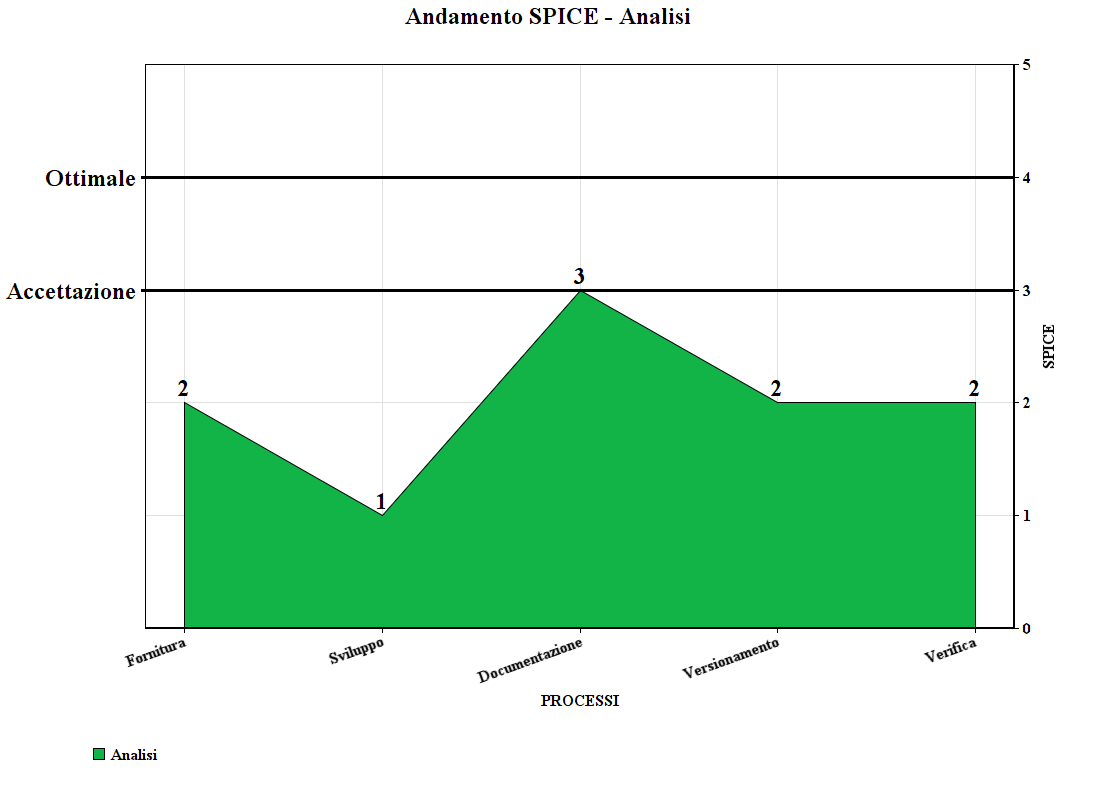
\includegraphics[scale=0.5]{verifica-analisi-spice}
	\centering
	\caption{Andamento dei valori SPICE, periodo di Analisi}
\end{figure}

\subsection{Prodotti}

\subsubsection{Documenti}

Segue riassunto del calcolo dell'Indice Gulpease [MPPD002] (al netto di tabelle e frontespizio) e di quello del numero di Errori ortografici corretti [MPPD001].

\begin{itemize}
	\item \textbf{Errori ortografici corretti [MPPD001]}: tramite le funzionalità di rilevazione d'errori di TexStudio sono stati rilevati e corretti complessivamente 14 errori all'interno dei documenti;
	
	\item \textbf{Indice Gulpease [MPPD002]}: Viene qui riportata una tabella contenente il valore Gulpease calcolato per ciascun documento.
	Per il calcolo di tale indice sono state escluse eventuali tabelle presenti nei documenti, le pagine di frontespizio e i diari delle modifiche, in quanto una loro inclusione avrebbe portato a valori errati. L'esito della misurazione è Positivo, se l'indice è maggiore o uguale a 50, o Negativo nel caso fosse inferiore a tale valore.
	
	\begin{table}[h]
		\begin{center}
			\setlength\LTleft{6mm}
			\begin{longtable}{|p{60mm}|p{30mm}|p{25mm}|}
				\hline  
				\textbf{Nome Documento} & \textbf{Valore Indice} & \textbf{Esito} \\ \hline    
				\textit{Glossario v 1.0.0} & 55 & Positivo\\ \hline    
				\textit{Norme di Progetto v 1.0.0} & 56 & Positivo\\ \hline    
				\textit{Studio di Fattibilità v 1.0.0} & 58 & Positivo\\ \hline    
				\textit{Piano di Progetto v 1.0.0} & 53 & Positivo\\ \hline    
				\textit{Analisi dei Requisiti v 1.0.0} & 55 & Positivo\\ \hline    
				\textit{Piano di Qualifica v 1.0.0} & 55 & Positivo\\ \hline    
				\textit{Verbale Interno 10-11-2017} & 55 & Positivo\\ \hline    
				\textit{Verbale Interno 1-12-2017} & 53 & Positivo\\ \hline    
				\textit{Verbale Esterno 15-12-2017} & 57 & Positivo\\ \hline    
				\textit{Verbale Esterno 3-01-2018} & 51 & Positivo\\ \hline   
				\textit{Lettera di Presentazione} & 80 & Positivo\\ \hline
			\end{longtable}
		\end{center}
		\caption{Valori Indice Gulpease, periodo di Analisi} 
	\end{table} 
	
	\begin{figure}[H]
		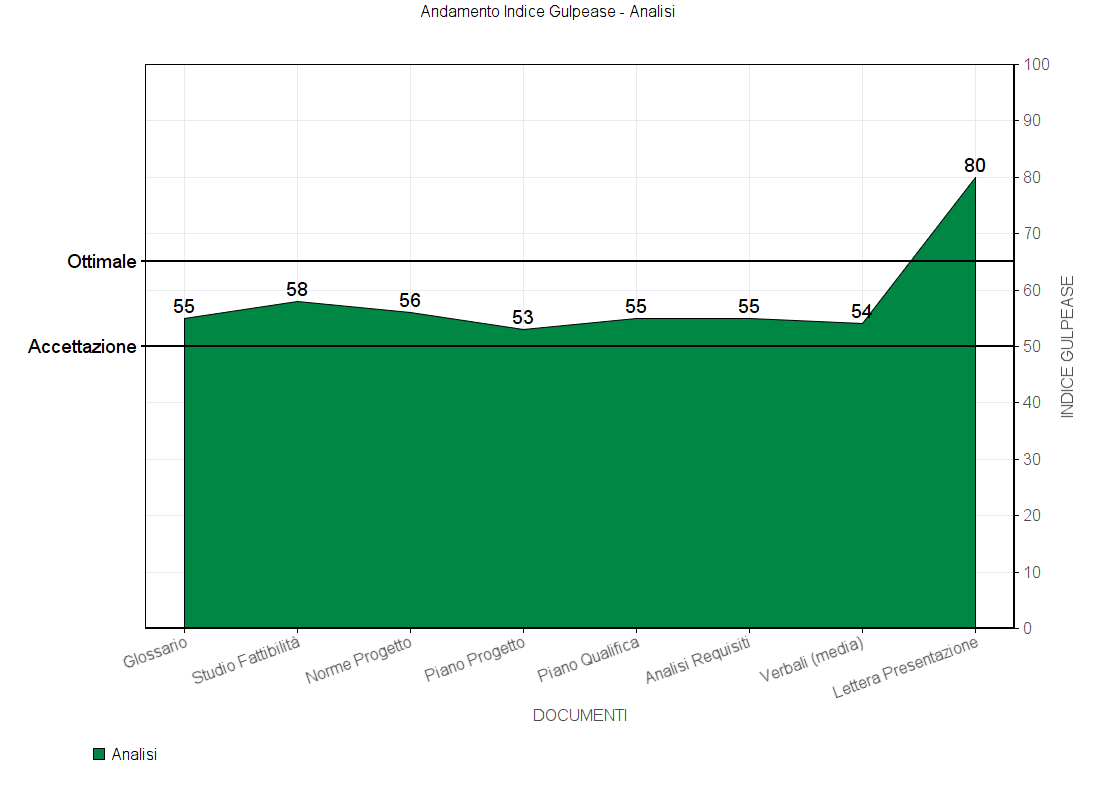
\includegraphics[scale=0.5]{verifica-analisi-gulpease}
		\centering
		\caption{Andamento dei valori Indice Gulpease, periodo di Analisi}
	\end{figure}
		
	Dalla tabella e dal grafico si evince che tutti i documenti presentano un indice nei limiti preferibili.

\end{itemize}

% CONSOLIDAMENTO

\section{Consolidamento requisiti e tecnologie}

\subsection{Processi}

L'applicazione del miglioramento continuo e la profonda revisione delle NP, concretizzatasi nel documento \textit{Norme di Progetto v2.0.0}, ha portato al miglioramento di seguito illustrato:

\newpage

\begin{table}[h]
	\begin{center}
		\setlength\LTleft{-22mm}
		\begin{longtable}{|p{35mm}|p{20mm}|p{20mm}|p{20mm}|p{20mm}|p{20mm}|p{20mm}|}
			\hline
			\textbf{Nome Processo} & \textbf{Attr. L1} & \textbf{Attr. L2} & \textbf{Attr. L3} & \textbf{Attr. L4} & \textbf{Attr. L5} & \textbf{SPICE}\\
			\hline
			\multirow{2}{*}{\textit{Fornitura}} & \multirow{2}{*}{PP: F} & PM: F & PDEF: F & PMS: P & PCH: N & Inizio: 0\\  
			\cline{3-7}
			&          & WPM: F & PDIS: F & PC: N & PI: N & Fine: 3 \\ 
			\hline
			\multirow{2}{*}{\textit{Sviluppo}} & \multirow{2}{*}{PP: F} & PM: F & PDEF: F & PMS: N & PCH: N & Inizio: 0\\  \cline{3-7}
			&          & WPM: F & PDIS: N & PC: N & PI: N & Fine: 2\\
			\hline\multirow{2}{*}{\textit{Documentazione}} & \multirow{2}{*}{PP: F} & PM: F & PDEF: F & PMS: F & PCH: P & Inizio: 0\\  \cline{3-7}
			&          & WPM: F & PDIS: F & PC: L & PI: N & Fine: 4\\ 
			\hline\multirow{2}{*}{\textit{Versionamento}} & \multirow{2}{*}{PP: F} & PM: F & PDEF: F & PMS: P & PCH: N & Inizio: 0\\  \cline{3-7}
			&          & WPM: F & PDIS: F & PC: P & PI: N & Fine: 3\\ 
			\hline\multirow{2}{*}{\textit{Verifica}} & \multirow{2}{*}{PP: F} & PM: F & PDEF: L & PMS: P & PCH: N & Inizio: 0\\  \cline{3-7}
			&          & WPM: F & PDIS: L & PC: N & PI: N & Fine: 3\\ 
			\hline       
		\end{longtable}
	\end{center}
	\caption{Valori SPICE, periodo di Consolidamento requisiti e tecnologie} 
\end{table}

\begin{figure}[H]
	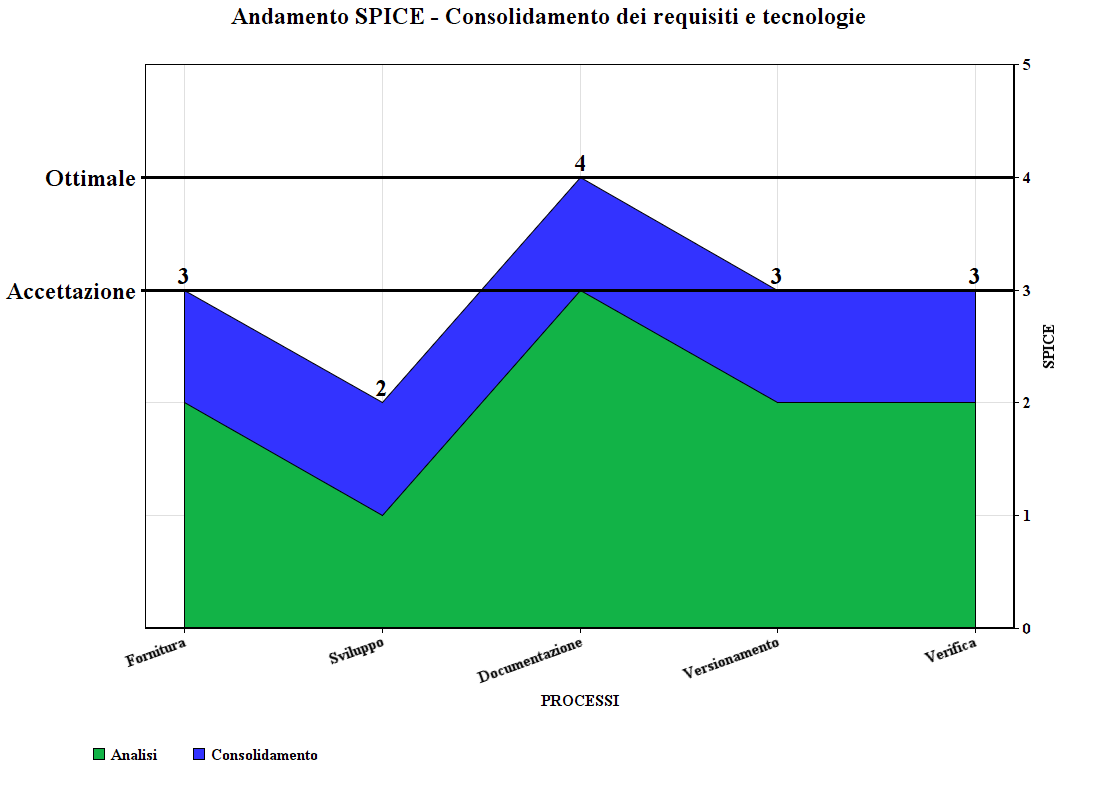
\includegraphics[scale=0.5]{verifica-consolidamento-spice}
	\centering
	\caption{Andamento dei valori SPICE, periodo di Consolidamento requisiti e tecnologie}
\end{figure}

\subsection{Prodotti}

\subsubsection{Documenti}

Segue riassunto del calcolo dell'Indice Gulpease [MPPD002] (al netto di tabelle e frontespizio) e di quello del numero di Errori ortografici corretti [MPPD001].

\begin{itemize}
	\item \textbf{Errori ortografici corretti [MPPD001]}: tramite le funzionalità di rilevazione d'errori di TexStudio sono stati rilevati e corretti complessivamente 23 errori all'interno dei documenti;
	
	\item \textbf{Indice Gulpease [MPPD002]}: Viene qui riportata una tabella contenente il valore Gulpease calcolato per ciascun documento.
	Per il calcolo di tale indice sono state escluse eventuali tabelle presenti nei documenti, le pagine di frontespizio e i diari delle modifiche, in quanto una loro inclusione avrebbe portato a valori errati. L'esito della misurazione è Positivo, se l'indice è maggiore o uguale a 50, o Negativo nel caso fosse inferiore a tale valore.
	
	\begin{table}[h]
		\begin{center}
			\setlength\LTleft{6mm}
			\begin{longtable}{|p{60mm}|p{30mm}|p{25mm}|}
				\hline  
				\textbf{Nome Documento} & \textbf{Valore Indice} & \textbf{Esito} \\ \hline    
				\textit{Glossario v 2.0.0} & 55 & Positivo\\ \hline    
				\textit{Norme di Progetto v 2.0.0} & 59 & Positivo\\ \hline    
				\textit{Piano di Progetto v 2.0.0} & 55 & Positivo\\ \hline    
				\textit{Analisi dei Requisiti v 2.0.0} & 58 & Positivo\\ \hline    
				\textit{Piano di Qualifica v 2.0.0} & 56 & Positivo\\ \hline    
				\textit{Verbale Interno 2018-29-01} & 57 & Positivo\\ \hline
				\textit{Verbale Esterno 2018-08-02} & 55 & Positivo\\ \hline
				\textit{Verbale Interno 2018-01-03} & 53 & Positivo\\ \hline    
				\textit{Lettera di Presentazione} & 80 & Positivo\\ \hline
			\end{longtable}
		\end{center}
		\caption{Valori Indice Gulpease, periodo di Consolidamento requisiti e tecnologie} 
	\end{table} 
	
	\begin{figure}[H]
		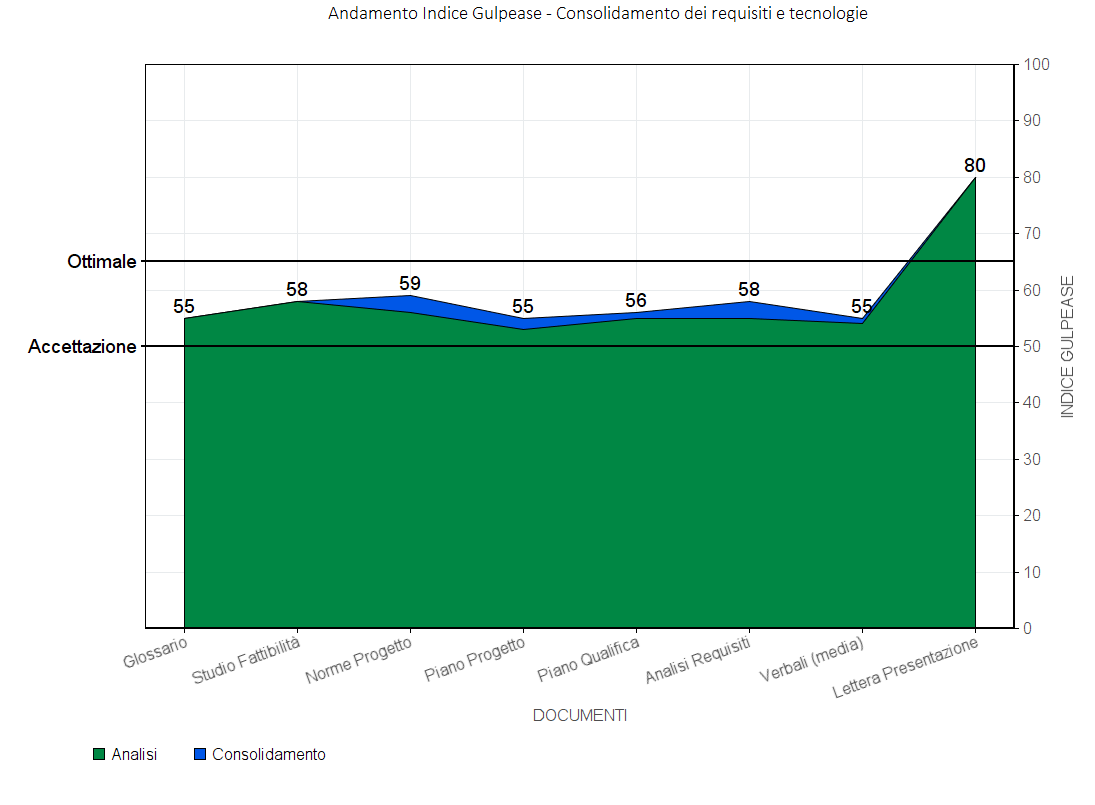
\includegraphics[scale=0.5]{verifica-consolidamento-gulpease}
		\centering
		\caption{Andamento dei valori Indice Gulpease, periodo di Consolidamento}
	\end{figure}
	
	Dalla tabella e dal grafico si evince che tutti i documenti presentano un indice nei limiti preferibili.	
\end{itemize}

%PROGETTAZIONE E CODIFICA

\section{Progettazione e codifica}

\subsection{Processi}

A seguito di numerosi miglioramenti apportati durante la revisione delle NP, giunta alla redazione del documento \textit{Norme di Progetto v3.0.0}, sono stati apportati ulteriori miglioramenti nello svolgimento dei processi visibili nella tabella sottostante

\newpage

\begin{table}[h]
	\begin{center}
		\setlength\LTleft{-22mm}
		\begin{longtable}{|p{35mm}|p{20mm}|p{20mm}|p{20mm}|p{20mm}|p{20mm}|p{20mm}|}
			\hline
			\textbf{Nome Processo} & \textbf{Attr. L1} & \textbf{Attr. L2} & \textbf{Attr. L3} & \textbf{Attr. L4} & \textbf{Attr. L5} & \textbf{SPICE}\\
			\hline
			\multirow{2}{*}{\textit{Fornitura}} & \multirow{2}{*}{PP: F} & PM: F & PDEF: F & PMS: P & PCH: P & Inizio: 3\\  
			\cline{3-7}
			&          & WPM: F & PDIS: F & PC: P & PI: P & Fine: 4 \\ 
			\hline
			\multirow{2}{*}{\textit{Sviluppo}} & \multirow{2}{*}{PP: F} & PM: F & PDEF: F & PMS: P & PCH: P & Inizio: 2\\  \cline{3-7}
			&          & WPM: F & PDIS: N & PC: N & PI: N & Fine: 3\\
			\hline\multirow{2}{*}{\textit{Documentazione}} & \multirow{2}{*}{PP: F} & PM: F & PDEF: F & PMS: F & PCH: P & Inizio: 4\\  \cline{3-7}
			&          & WPM: F & PDIS: F & PC: L & PI: P & Fine: 4\\ 
			\hline\multirow{2}{*}{\textit{Versionamento}} & \multirow{2}{*}{PP: F} & PM: F & PDEF: F & PMS: P & PCH: P & Inizio: 3\\  \cline{3-7}
			&          & WPM: F & PDIS: F & PC: P & PI: P & Fine: 4\\ 
			\hline\multirow{2}{*}{\textit{Verifica}} & \multirow{2}{*}{PP: F} & PM: F & PDEF: L & PMS: P & PCH: P & Inizio: 3\\  \cline{3-7}
			&          & WPM: F & PDIS: L & PC: P & PI: P & Fine: 3\\ 
			\hline       
		\end{longtable}
	\end{center}
	\caption{Valori SPICE, periodo di Progettazione e codifica} 
\end{table}

\begin{figure}[H]
	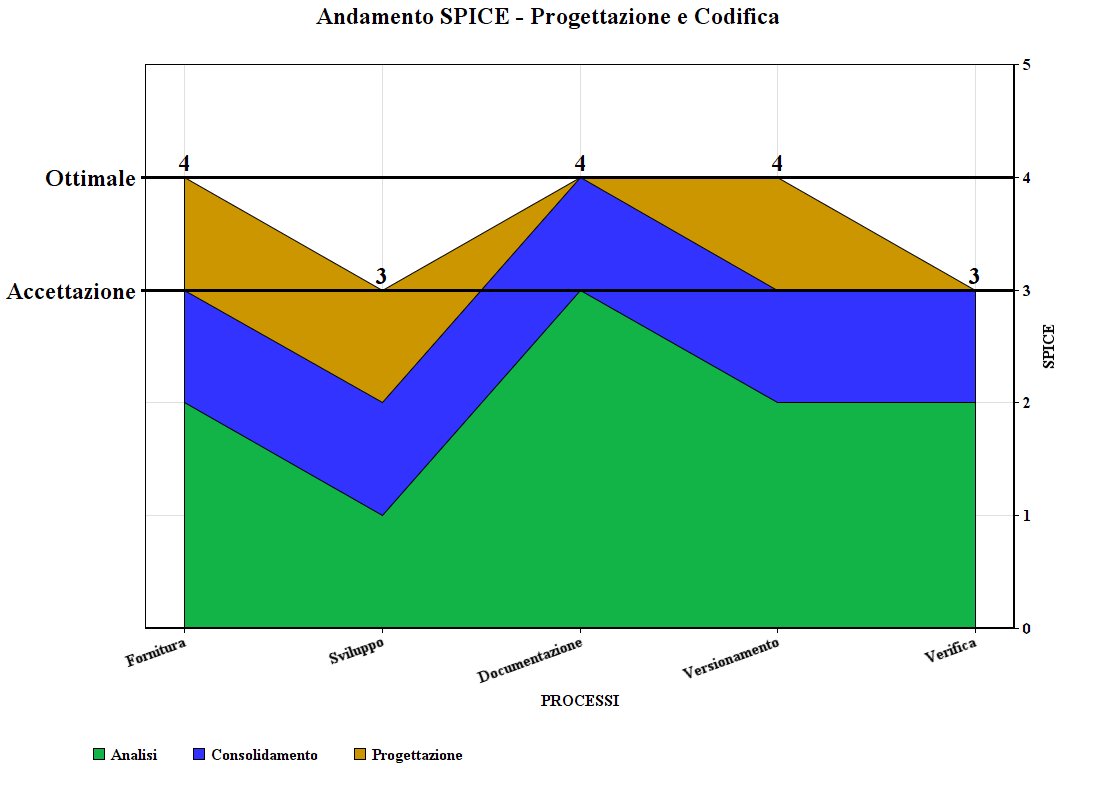
\includegraphics[scale=0.5]{verifica-progettazione-spice}
	\centering
	\caption{Andamento dei valori SPICE, periodo di Progettazione e codifica}
\end{figure}

\subsection{Prodotti}

\subsubsection{Documenti}

Segue riassunto del calcolo dell'Indice Gulpease [MPPD002] (al netto di tabelle e frontespizio) e di quello del numero di Errori ortografici corretti [MPPD001].

\begin{itemize}
	\item \textbf{Errori ortografici corretti [MPPD001]}: tramite le funzionalità di rilevazione d'errori di TexStudio sono stati rilevati e corretti complessivamente 17 errori all'interno dei documenti;
	
	\item \textbf{Indice Gulpease [MPPD002]}: Viene qui riportata una tabella contenente il valore Gulpease calcolato per ciascun documento.
	Per il calcolo di tale indice sono state escluse eventuali tabelle presenti nei documenti, le pagine di frontespizio e i diari delle modifiche, in quanto una loro inclusione avrebbe portato a valori errati. L'esito della misurazione è Positivo, se l'indice è maggiore o uguale a 50, o Negativo nel caso fosse inferiore a tale valore.
	
	\begin{table}[h]
		\begin{center}
			\setlength\LTleft{6mm}
			\begin{longtable}{|p{60mm}|p{30mm}|p{25mm}|}
				\hline  
				\textbf{Nome Documento} & \textbf{Valore Indice} & \textbf{Esito} \\ \hline    
				\textit{Glossario v 3.0.0} & 56 & Positivo\\ \hline    
				\textit{Norme di Progetto v 3.0.0} & 59 & Positivo\\ \hline    
				\textit{Piano di Progetto v 3.0.0} & 57 & Positivo\\ \hline    
				\textit{Analisi dei Requisiti v 3.0.0} & 60 & Positivo\\ \hline    
				\textit{Piano di Qualifica v 3.0.0} & 58 & Positivo\\ \hline    
				\textit{Verbale Esterno 2018-03-17} & 54 & Positivo\\ \hline
				\textit{Verbale Interno 2018-03-21} & 55 & Positivo\\ \hline
				\textit{Verbale Interno 2018-03-29} & 54 & Positivo\\ \hline
				\textit{Verbale Interno 2018-04-02} & 59 & Positivo\\ \hline
				\textit{Verbale Esterno 2018-04-06} & 53 & Positivo\\ \hline    
				\textit{Verbale Interno 2018-04-09} & 55 & Positivo\\ \hline
				\textit{Verbale Interno 2018-04-14} & 56 & Positivo\\ \hline
				\textit{Lettera di Presentazione} & 80 & Positivo\\ \hline
			\end{longtable}
		\end{center}
		\caption{Valori Indice Gulpease, periodo di Progettazione e codifica} 
	\end{table} 
	
	\begin{figure}[H]
		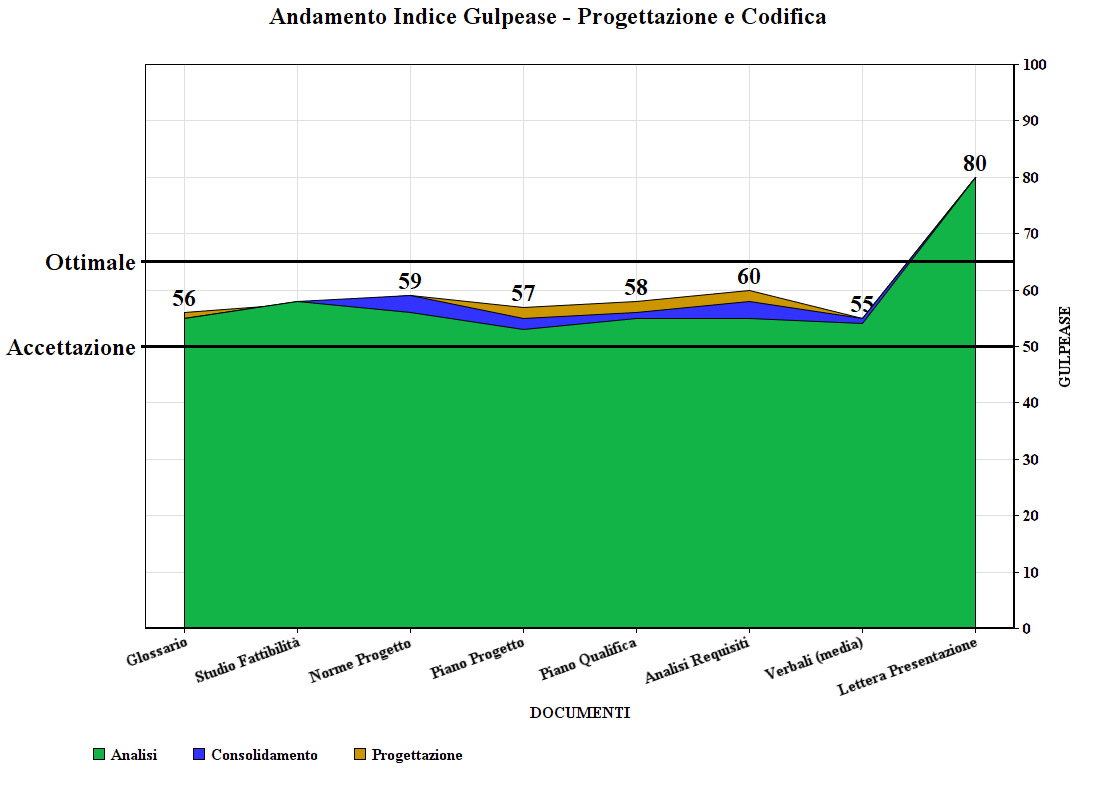
\includegraphics[scale=0.5]{verifica-progettazione-gulpease}
		\centering
		\caption{Andamento dei valori Indice Gulpease, periodo di Progettazione e codifica}
	\end{figure}
	
	Dalla tabella e dal grafico si evince che tutti i documenti presentano un indice nei limiti preferibili.	
\end{itemize}

%\subsubsection{Software}

\chapter{Valutazioni per il miglioramento}

\section{Introduzione}

Questa appendice si propone di riepilogare le valutazioni orientate al miglioramento dell'intero processo produttivo in relazione al progetto corrente. Verranno dunque tracciati problemi riguardanti i seguenti ambiti:

\begin{itemize}
	\item \textbf{Organizzazione:} ovvero quei problemi inerenti l'organizzazione e la comunicazione all'interno del gruppo;
	\item \textbf{Ruoli:} ovvero quei problemi riguardanti il corretto svolgimento di un ruolo di progetto;
	\item \textbf{Strumenti:} ovvero quei problemi riguardanti il corretto utilizzo di strumentazione specifica.
\end{itemize}

\noindent Ogni problema viene sollevato sulla base dell'autovalutazione dei membri del gruppo e dall'esito di revisioni e confronti con Committente e Proponente, e ad esso viene associata una possibile soluzione.

\section{Valutazioni sull'organizzazione}
\begin{itemize}
	\item \textbf{Problema}: Difficoltà nel conciliare gli impegni dei membri del gruppo nel contesto dell'organizzazione di riunioni e confronti fisici. \\ \\
	\textbf{Soluzione} Per garantire lo svolgimento di riunioni ed incontri si è optato per l'utilizzo di strumenti per la messaggistica instantanea e videochiamate, che ha garantito una maggiore partecipazione dei membri.
\end{itemize}

\section{Valutazioni sui ruoli}

\subsection{Responsabile}

\begin{itemize}
	\item \textbf{Problema}: Difficoltà nella suddivisione equa del lavoro e dell'individuazione di task dal carico adeguato. \\ \\
	\textbf{Soluzione} Per bilanciare la suddivisione del lavoro si è deciso di individuare periodicamente un nuovo insieme relativamente ristretto di task di entità ridotta.
\end{itemize}

\subsection{Analista}

\begin{itemize}
	\item \textbf{Problema}: Difficoltà nell'individuazione e corretta classificazione dei requisiti. \\ \\
	\textbf{Soluzione} Per garantire un buon esito dell'attività di analisi si è condiviso maggiormente il lavoro tra gli Analisti, sfruttando i vari mezzi scelti per la comunicazione
	all'interno del gruppo per generare maggiore confronto.
\end{itemize}

\subsection{Verificatore}

\begin{itemize}
	\item \textbf{Problema}: Difficoltà nell'analisi approfondita dei documenti per verificarne correttezza e completezza da parte di membri relativamente estranei allo specifico documento. \\ \\
	\textbf{Soluzione} Per garantire la buona riuscita della verifica e validazione si è scelto di dedicarvi maggiori risorse temporali.
\end{itemize}

\section{Valutazioni sugli strumenti}

\begin{itemize}
	\item \textbf{Problema}: A causa dell'inesperienza del gruppo si è mostrata iniziale difficoltà nell'ottenere padronanza degli strumenti selezionati. \\ \\
	\textbf{Soluzione} I membri del gruppo più esperti hanno condiviso la maggiore conoscenza degli strumenti. Una parte adeguata di tempo è stata dedicata al confronto su questo tema, a domande, consigli e produzione di piccole guide riassuntive sugli strumenti in uso.
\end{itemize}

\chapter{Esiti delle revisioni}

In questa appendice vengono indicate le modifiche apportate dal gruppo al proprio way of working, alle proprie strategie e ai propri documenti formali a seguito degli esiti delle revisioni.

\section{Revisione dei Requisiti}

A seguito dell'esito della Revisione dei Requisiti sono state apportate le seguenti modifiche:

\begin{itemize}
	\item Eliminata a livello normativo l’ambiguità tra prodotti e processi e chiarita la relazione tra processi primari e di supporto. In particolare, normata in maniera più dettagliata la gestione di progetto;
	\item Ampliamento del dettaglio dei requisiti, ora supportati da diagrammi più precisi ed efficaci;
	\item Ristrutturazione profonda dei documenti in base al feedback ricevuto:
	\begin{itemize}
		\item \textbf{Norme di Progetto}: Ristrutturato il documento eliminando l'ambiguità tra processi e documenti da essi prodotti. Vengono ora normati i processi di supporto di gestione della qualità e gestione di progetto e quelli organizzativi di formazione del personale e miglioramento continuo. Aumentata in generale la profondità dei contenuti e introdotti diagrammi descrittivi delle procedure;
		\item \textbf{Piano di Progetto}: Rivisto il ciclo di sviluppo incrementale e ristrutturata contestualmente la pianificazione. Incrementata la leggibilità dell'analisi dei rischi mediante forme tabellari;
		\item \textbf{Piano di Qualifica}: Eliminata l'ambiguità con alcuni elementi attinenti alle NP e definiti più chiaramente obiettivi di qualità e soglie metriche. Introdotte inoltre le appendici inerenti test e valutazioni per il miglioramento;
		\item \textbf{Analisi dei Requisiti}: Dettagliati maggiormente requisiti e use case apportando contestualmente modifiche migliorative ai diagrammi errati.
	\end{itemize}
\end{itemize}

\section{Revisione di Progettazione}

A seguito dell'esito della Revisione di Progettazione sono state apportate le seguenti modifiche:

\begin{itemize}
	\item Ristrutturazione profonda dei documenti in base al feedback ricevuto:
	\begin{itemize}
		\item \textbf{Norme di Progetto}: correzione di errori di digitazione e grammaticali. Aggiunta contenuti precedentemente presenti nel PdQ. Precisazione dell'insieme di comportamenti da adottare per il conseguimento dei requisiti di qualità e miglioramento della definizione di validazione;
		\item \textbf{Piano di Progetto}: aggiunta tipologia di rischi e riscontri effettuati nella fase di progettazione. Corretti alcuni errori nell'uso poco oculato di alcuni termini all'interno del documento;
		\item \textbf{Piano di Qualifica}: rimozione contenuti non attinenti al documento;
		\item \textbf{Analisi dei Requisiti}: risoluzione problemi di compilazione e correzione nella descrizione di alcuni casi d'uso.
	\end{itemize}
\end{itemize}

\end{document}
